\documentclass[12pt,a4paper]{report}
\usepackage[utf8]{inputenc}
\usepackage[T1]{fontenc}
\usepackage{geometry}
\geometry{a4paper, margin=2.5cm}
\usepackage{setspace}
\onehalfspacing
\usepackage{graphicx}
\usepackage{pdfpages}
\usepackage{booktabs}
\usepackage{array}
\usepackage{longtable}
% Full-grid table style — compact, consistent spacing
\setlength{\arrayrulewidth}{0.8pt}
\renewcommand{\arraystretch}{1.1}
\setlength{\tabcolsep}{4.5pt}
\usepackage{hyperref}
\hypersetup{
  colorlinks=true,
  linkcolor=blue,
  citecolor=blue,
  urlcolor=black,
  filecolor=blue
}
\usepackage{microtype}
\usepackage{amsmath}
\usepackage{float}
\usepackage{caption}
\usepackage{subcaption}
\usepackage{fancyhdr}
\usepackage{titlesec}
\usepackage{parskip}
\setlength{\parskip}{9pt plus 2pt minus 1pt}
\usepackage[table]{xcolor}
\usepackage{multirow}
\usepackage{listings}
\usepackage{tikz}
\usetikzlibrary{patterns, calc}

\lstset{
  basicstyle=\ttfamily\small,
  backgroundcolor=\color{gray!10},
  frame=single, breaklines=true,
  keywordstyle=\color{blue},
  commentstyle=\color{green!60!black},
  stringstyle=\color{red!70!black},
}

\graphicspath{{figures/}{run_graphs/}{run_graphs/ThermalDroneNet/}}

\pagestyle{fancy}
\fancyhf{}
\lhead{\small \leftmark}
\cfoot{\thepage}

% Suppress header/footer on blank pages inserted by cleardoublepage
\makeatletter
\def\cleardoublepage{\clearpage\if@twoside\ifodd\c@page\else
  \hbox{}\thispagestyle{empty}\newpage\fi\fi}
\makeatother

% Allow slightly loose line breaking to prevent overfull hboxes
\sloppy
\tolerance=1000
\emergencystretch=3em
\hyphenpenalty=1000
\exhyphenpenalty=1000

% ---- Body text: 12pt Times New Roman with 1.5 line spacing ----
\usepackage{mathptmx} % Times New Roman font
\renewcommand{\normalsize}{\fontsize{12}{18}\selectfont}
\normalsize

% ---- Paragraphs: block style with spacing between paragraphs ----
\usepackage{indentfirst}
\setlength{\parindent}{0pt}

% ---- Heading hierarchy: UofK EE standard sizes ----
\titleformat{\chapter}[display]
{\normalfont\fontsize{16}{19.2}\bfseries\centering}{\chaptertitlename\ \thechapter}{20pt}{\fontsize{18}{21.6}\bfseries}
\titlespacing*{\chapter}{0cm}{50pt}{40pt}

\titleformat{\section}
{\normalfont\fontsize{14}{16.8}\bfseries}{\thesection}{1em}{}
\titlespacing*{\section}{0cm}{20pt}{10pt}

\titleformat{\subsection}
{\normalfont\fontsize{12}{14.4}\bfseries}{\thesubsection}{1em}{}
\titlespacing*{\subsection}{0cm}{16pt}{8pt}

\titleformat{\subsubsection}
{\normalfont\fontsize{12}{14.4}\bfseries\itshape}{\thesubsubsection}{1em}{}
\titlespacing*{\subsubsection}{0cm}{14pt}{6pt}

\begin{document}

\begin{titlepage}
  \centering
  \vspace*{0.5cm}
  \includegraphics[height=4.5cm]{logo.jpg}\\[0.6cm]
  {\scshape\LARGE University of Khartoum \par}
  \vspace{0.4cm}
  {\scshape\large Faculty of Engineering \par}
  \vspace{0.2cm}
  {\scshape\large Department of Electrical and Electronics Engineering \par}
  \vspace{1.8cm}
  {\LARGE\bfseries AI Multi-Agent Anti-UAV Detection System\par}
  \vspace{0.4cm}
  {\large\itshape A Distributed Edge-Computing Framework for Real-Time Anti-UAV Detection and Tracking\par}
  \vspace{1.5cm}
  {\large
    \textit{\textbf{Authors:}}\\[0.3cm]
    Abdelsamad Abdalla Abdelsamad Abdalla (184048)\\
    Mustafa Mubarak Elsaeed Mustafa (184096)\\[0.5cm]
    \textit{\textbf{Supervisor:}}\\[0.3cm]
    D. Magdi Amen\\[0.8cm]
    August 2026\par
  }
  \vfill
\end{titlepage}

\thispagestyle{empty}
\vspace*{\fill}
\begin{center}
{\Large\bfseries Dedication}\\[1.5cm]
{\itshape To our families, whose endless support and patience made this journey possible.}
\end{center}
\vspace*{\fill}

\newpage
\thispagestyle{empty}
\vspace*{\fill}
\begin{center}
{\Large\bfseries Acknowledgments}\\[1.5cm]
\end{center}
\begin{flushleft}
\itshape
We would like to express our sincere gratitude to our supervisor, Dr. Magdi Amen, for his invaluable guidance and support throughout this project. We also thank the University of Khartoum's Department of Electrical and Electronic Engineering for providing the resources and environment that made this work possible. Finally, we thank our families and friends for their continuous encouragement.
\end{flushleft}
\vspace*{\fill}

\newpage
\thispagestyle{empty}
\includepdf[pages=-,fitpaper]{arabic.pdf}

\newpage
\thispagestyle{empty}
\begin{center}
\bfseries \abstractname
\end{center}
This report presents a comprehensive AI-powered distributed anti-UAV detection system that addresses a critical security challenge: distinguishing between drones and birds in real-time surveillance environments. The system combines cutting-edge deep learning with distributed edge computing to deliver accurate, scalable threat detection across multiple monitoring locations.

At the heart of the system is \textbf{BirdDroneNet}, a specialized YOLO26s-based detection model trained on 7,434 diverse images to differentiate between birds and drones: a challenge that has long plagued conventional single-class detectors. Through careful dataset curation and pseudo-label fine-tuning on complex real-world backgrounds, the model achieves exceptional performance: 94.6\% mean average precision with a remarkably low 0.3\% bird false alarm rate. The system demonstrates strong detection capabilities, achieving 88.9\% mAP on quadcopter UAV datasets, 95.2\% on bird datasets, and 52.7\% on fixed-wing UAV detection.

To extend detection capabilities beyond visible light, a dedicated \textbf{ThermalDroneNet} model was developed for thermal infrared surveillance. Trained on 3,788 thermal images spanning diverse environmental conditions, this model achieves 95.8\% mean average precision on validation data and maintains over 90\% precision on the challenging Anti-UAV410 benchmark, demonstrating the system's adaptability to night-time and adverse weather conditions where RGB cameras fall short.

The distributed architecture enables seamless coordination of multiple edge detection nodes through a sophisticated web-based control center. This central platform provides secure authentication, real-time monitoring dashboards with intuitive color-coded threat visualization, interactive geographic mapping of device locations, and live video streaming. The system's modular design ensures scalability from small installations to large-scale deployments without architectural modifications.

Together, these contributions establish a practical, deployable solution for UAV threat detection that bridges the gap between academic research and real-world operational requirements. The system is built entirely on publicly available datasets and open-source frameworks, ensuring reproducibility and facilitating further research in this rapidly evolving field.

\pagenumbering{roman}
\setcounter{page}{1}
\tableofcontents
\listoffigures
\listoftables

\newpage
\section*{List of Abbreviations}
\addcontentsline{toc}{section}{List of Abbreviations}

\begin{longtable}{@{}p{3.2cm}@{}p{11cm}@{}}
ADAS      & Advanced Driver Assistance System \\
API       & Application Programming Interface \\
CCTV      & Closed-Circuit Television \\
CLAHE     & Contrast Limited Adaptive Histogram Equalisation \\
CNN       & Convolutional Neural Network \\
COCO      & Common Objects in Context (benchmark dataset) \\
CPU       & Central Processing Unit \\
CC0       & Creative Commons Zero (public domain licence) \\
DETR      & Detection Transformer \\
DFL       & Distribution Focal Loss \\
DR        & Detection Rate \\
DUT       & Dalian University of Technology (Anti-UAV dataset) \\
FAR       & False Alarm Rate \\
FLIR      & Forward-Looking Infrared \\
FOV       & Field of View \\
FP        & False Positive \\
FN        & False Negative \\
GPU       & Graphics Processing Unit \\
HSV       & Hue, Saturation, Value (colour space) \\
ICE       & Interactive Connectivity Establishment \\
INT8      & 8-bit Integer (quantisation format) \\
JSON      & JavaScript Object Notation \\
JWT       & JSON Web Token \\
KFUPM     & King Fahd University of Petroleum and Minerals \\
LAN       & Local Area Network \\
LWIR      & Long-Wave Infrared \\
mAP       & Mean Average Precision \\
MQTT      & Message Queuing Telemetry Transport \\
NAT       & Network Address Translation \\
NMS       & Non-Maximum Suppression \\
PTZ       & Pan-Tilt-Zoom \\
RCNN      & Region-based Convolutional Neural Network \\
SDP       & Session Description Protocol \\
SGD       & Stochastic Gradient Descent \\
SIDD      & Shandong Infrared Drone Dataset \\
SIRST     & Single-Frame Infrared Small Target \\
STAL      & Small-Target-Aware Label Assignment \\
TLS       & Transport Layer Security \\
TN        & True Negative \\
TP        & True Positive \\
TURN      & Traversal Using Relays around NAT \\
UAS       & Unmanned Aerial System \\
UAV       & Unmanned Aerial Vehicle \\
WebRTC    & Web Real-Time Communication \\
\end{longtable}

\cleardoublepage
\pagenumbering{arabic}
\setcounter{page}{1}

% ============================================================
\chapter{Introduction}

\section{Background of the Study}

In recent years, electrical and computer engineering systems have experienced
significant technological advancements, particularly in the areas of artificial
intelligence, computer vision, and distributed embedded computing. Unmanned
aerial vehicles (UAVs), commonly known as drones, have proliferated rapidly
across both consumer and commercial markets. Originally confined to military
applications, UAVs are now widely used in photography, agriculture, logistics,
and infrastructure inspection.

This technological democratisation has, however, introduced serious security
challenges. Consumer drones are increasingly exploited for surveillance,
smuggling, and attacks on critical infrastructure. Airports, power stations,
government facilities, and public events are all vulnerable to unauthorised
UAV incursions. Vision-based anti-UAV detection systems have emerged as a
cost-effective countermeasure, leveraging advances in deep learning object
detection to identify and track aerial threats in real time.

A key challenge in vision-based UAV detection is the visual similarity
between drones and birds at long range. Both occupy the same low-altitude
airspace, exhibit similar apparent sizes at distance, and move in comparable
flight patterns. Distinguishing between them is the central technical problem
that this project addresses.

\section{Problem Statement}

Existing anti-UAV detection systems suffer from three principal limitations.
First, single-class drone detectors do not distinguish between drones and
birds, leading to high false alarm rates in environments with bird activity.
Second, models trained on clean benchmark datasets degrade significantly
when deployed on real-world sequences with complex backgrounds such as
urban structures, tree canopies, and sky gradients. Third, most published
systems operate as standalone detectors without a distributed architecture
that allows multiple edge nodes to be monitored and controlled from a
centralised interface.

These limitations reduce the operational utility of existing systems:
a detector that generates frequent false alarms on birds will be disabled
by operators, and a system that cannot be monitored centrally cannot be
deployed at scale across a protected perimeter.

\section{Significance of the Project}

This project contributes to the field of airspace security and intelligent
embedded systems in the following ways:

\begin{itemize}
  \item \textbf{Academic contribution}: Demonstrates a complete pipeline
        from dataset curation and model training to real-world evaluation
        on the DUT Anti-UAV benchmark, providing reproducible baselines
        for the Bird/Drone discrimination task.
  \item \textbf{Practical contribution}: Delivers a deployable distributed
        detection system with a web-based control center, enabling real-time
        monitoring of multiple edge nodes from a single interface.
  \item \textbf{Technical contribution}: Introduces a pseudo-label fine-tuning
        methodology that improves detection continuity on real-world sequences
        without requiring manual annotation of the fine-tuning data.
\end{itemize}

\section{Project Objectives}

The general objective of this project is to design, implement, and evaluate
an AI-powered distributed anti-UAV detection system capable of real-time
bird/drone discrimination on edge hardware with centralised web-based monitoring.

The specific objectives are:

\begin{enumerate}
  \item Design and implement a 2-class aerial object detection model (Bird, Drone)
        using YOLO26s, trained on curated RGB datasets with balanced class representation.
  \item Fine-tune the detection model on supplementary aerial datasets to improve
        real-world detection continuity and reduce false positives on complex backgrounds.
  \item Implement a distributed edge-computing inference pipeline with
        MQTT communication, WebRTC live streaming, and PTZ camera control.
  \item Design and implement a web-based control center with JWT authentication,
        real-time monitoring, and multi-device management.
  \item Train and evaluate a dedicated thermal infrared detection model,
        to establish a thermal detection baseline for 24/7 operation.
\end{enumerate}

\section{Scope and Limitations}

\begin{itemize}
  \item Training datasets are limited to publicly available RGB drone and
        bird imagery (CC BY 4.0 and CC0 licenses).
  \item The DUT Anti-UAV evaluation uses proxy metrics (detection rate,
        tracking gaps) since per-frame annotations are not available in
        the tracking split.
  \item The system is evaluated primarily under normal lighting conditions;
        training data diversity was extended through Roboflow augmentation
        pipelines simulating varied weather and lighting conditions
        (brightness, contrast, blur, noise, and hue shifts), providing
        partial robustness coverage without requiring real adverse-weather
        captures.
\end{itemize}

The thermal infrared gap deserves specific mention. Delleji et al.~\cite{delleji2025thermal}
highlight a critical deficiency in existing public thermal datasets for aerial drone detection.
Specifically:
\begin{itemize}
  \item The FLIR ADAS dataset is designed for automotive scenes and is not applicable to aerial detection.
  \item The KAIST Multispectral dataset focuses on pedestrian detection, not aerial targets.
  \item Available aerial thermal datasets contain fewer than 2,000 frames with minimal scene diversity.
\end{itemize}
Their work further demonstrates that a custom thermal acquisition pipeline (capturing three
DJI UAV types at multiple altitudes with a 640$\times$512 LWIR sensor) is necessary to
achieve reliable thermal detection. This confirms that extending the thermal modality beyond
the current SIDD-trained model requires a dedicated dataset acquisition effort that is outside
the scope of the present work.

\section{Methodology Overview}

The methodology follows four main stages: dataset curation and preparation,
model training and fine-tuning, system implementation, and performance
evaluation. Full implementation details are provided in Chapter~3.

\section{Report Structure}

Chapter~2 provides the theoretical background and literature review.
Chapter~3 describes the full methodology including requirements, system
framework, datasets, and implementation. Chapter~4 presents training and
evaluation results. Chapter~5 discusses the findings. Chapter~5 concludes
with deployment recommendations and future work.

% ============================================================
\chapter{Literature Review}

\section*{Part I: Theoretical Background}
\addcontentsline{toc}{section}{Part I: Theoretical Background}

\section{Fundamental Concepts}

This project draws on five established building blocks: single-stage
object detection (the YOLO paradigm and mean Average Precision as its
evaluation metric), transfer learning from COCO-pretrained backbones,
edge computing for co-located inference, MQTT for lightweight
publish-subscribe telemetry between edge nodes and the control center,
and WebRTC for low-latency live video streaming to operators. These
concepts are foundational rather than novel, so full definitions and
background explanations are provided in Appendix~\ref{app:theory} rather
than expanded here; the remainder of this chapter focuses on the
literature that is directly relevant to the system's design decisions.

\section{Related Systems and Models}

\subsection{Distributed Anti-UAV Detection Architectures}

A distributed anti-UAV system consists of multiple sensor nodes (cameras,
radars, or acoustic sensors) connected to a central command and control
system. Vision-based distributed systems use cameras at each node, running
local inference to reduce bandwidth requirements. The central system
aggregates detections, maintains a common operational picture, and allows
operators to task individual nodes (e.g., PTZ camera control).

The two-tier architecture adopted in this project (edge inference nodes
communicating over MQTT to a web-based control center) is consistent
with the distributed paradigm described in the literature. Each tier has
distinct responsibilities: the edge tier handles computationally intensive
inference, while the control tier handles aggregation, visualisation, and
operator interaction.

\subsection{YOLO-Based Aerial Object Detectors}

The YOLO family has been the dominant architecture for aerial object
detection since YOLOv3. Key variants relevant to this work include:
YOLOv5 (used in the KFUPM anti-UAV system~\cite{munir2023kfupm}), YOLOv8 (widely used in
aerial detection research), and YOLO26 (used in this project). Each
successive version improves small-object detection through architectural
changes to the feature pyramid network and label assignment strategy.

\section{Techniques, Methods, and Algorithms}

Three techniques from the wider literature are adapted directly in this
project's methodology: pseudo-label fine-tuning (using a trained model's
own confident predictions as training targets for a domain adaptation
stage), aerial-detection-specific data augmentation (copy-paste, rotation,
vertical flip, and mosaic, chosen for their effectiveness on small,
variably-oriented targets), and ByteTrack for multi-object tracking across
frames. Full descriptions of each technique are provided in
Appendix~
\ref{app:theory}; Section~\ref{sec:training_config} describes how each is specifically
configured and applied to the Bird/Drone detection task.

\section*{Part II: Literature Review}
\addcontentsline{toc}{section}{Part II: Literature Review}

\section{YOLO Model Family}

The YOLO (You Only Look Once) family of single-stage object detectors has
dominated real-time detection benchmarks since its introduction. YOLO26~\cite{ultralytics2025},
released by Ultralytics in September 2025, is a unified family of real-time
vision models that introduces native end-to-end inference and achieves
40.9--57.5 mAP on COCO at 1.7--11.8 ms T4 TensorRT latency across its five
detection scales.

YOLO26's design incorporates four key architectural areas relevant to aerial
UAV detection:

\begin{itemize}
  \item \textbf{Native end-to-end inference}: The default one-to-one detection
        head produces predictions without non-maximum suppression (NMS),
        simplifying deployment and reducing post-processing latency. Unlike
        traditional detectors that rely on NMS as a separate post-processing
        step, YOLO26 generates predictions directly, making production
        integration simpler and more efficient.
  
  \item \textbf{Lighter box regression (DFL-Free)}: YOLO26 removes Distribution
        Focal Loss (DFL), reducing detection-head complexity while preserving
        an unconstrained regression range. This simplification reduces model
        complexity without sacrificing accuracy.
  
  \item \textbf{MuSGD optimizer + Progressive Loss + STAL}: The training pipeline
        combines MuSGD (a hybrid Muon + SGD optimizer adapted from large language
        model training), Progressive Loss (which shifts training emphasis toward
        the inference-time head), and STAL (Small-Target-Aware Label Assignment)
        to improve optimization and maintain positive label coverage for small
        objects. STAL is particularly critical for aerial detection where drones
        occupy few pixels at distance.
  
  \item \textbf{Task-specific heads}: YOLO26 provides targeted designs for
        instance segmentation, pose estimation, and oriented detection while
        maintaining a single unified model pipeline across tasks.
\end{itemize}

\begin{figure}[H]
  \centering
  \includegraphics[width=\textwidth]{figures/yolo_family.png}
  \caption[YOLO family performance comparison]{YOLO family performance comparison. YOLO26 achieves state-of-the-art
  accuracy-latency trade-off, with the ``s'' variant (9.9M parameters) selected
  for this work due to its deployability on edge hardware and RTX 2070 compatibility.}
  \label{fig:yolo_family}
\end{figure}

YOLO26s (9.9M parameters, 22.5 GFLOPs) was selected for this work as it
fits within the RTX 2070 8GB VRAM budget at batch 16 (4.7GB peak) while
providing state-of-the-art accuracy for aerial imagery. The ``s'' (small)
variant is also deployable on edge hardware such as Raspberry Pi 4 and
NVIDIA Jetson Nano, making it suitable for the distributed inference
architecture of this system.


\section{UAV Detection Under Adverse Conditions}

Real-world anti-UAV systems must operate in conditions that deviate
significantly from the clean, well-lit imagery used in most benchmark
evaluations. Munir~\cite{munir2023kfupm} provides a systematic
study of UAV detection under adverse weather, with the following key findings:

\begin{itemize}
  \item Three weather-affected test sets were introduced: RTD (drizzle, heavy, and torrential rain),
        ANTD (low, medium, and high additive white Gaussian noise), and MBTD (low, medium, and high
        motion blur).
  \item YOLOv5m, the strongest baseline on clean data (mAP@0.5 = 95.6\%), degrades to 47.9\% under
        torrential rain and 21.9\% under high motion blur, drops of 50.6 and 77.0 percentage
        points respectively.
  \item YOLO-RAW, a multi-scale extension of YOLOv5, addresses this by adding a CBS+C3 block in the
        backbone, an SPPF-Enhanced module, four SimAM attention blocks in the neck, and a fourth P6
        prediction head. It achieves 95.2\% mAP@0.5 on the Complex Background Dataset.
  \item Training with weather-augmented data (33\% noisy + 33\% motion-blurred + 34\% rainy images)
        improves YOLOv5m's torrential rain performance from 47.9\% to 83.3\% mAP@0.5 and high-blur
        performance from 21.9\% to 66.8\%, with only a marginal drop on clean data (95.6\% to 94.6\%).
  \item This demonstrates that weather augmentation is a low-cost, high-impact robustness strategy
        directly applicable to YOLO26s training.
\end{itemize}

\section{Transfer Learning for Aerial Object Detection}

Transfer learning from large-scale detection models to domain-specific
aerial datasets has emerged as the dominant training paradigm for UAV
detection. Key findings from the literature include:

\begin{itemize}
  \item Reis et al.~\cite{reis2024yolov8} demonstrate a two-stage strategy: a generalised YOLOv8
        model trained on 15,064 images across 40 flying object classes (mAP@0.5 = 79.2\%) is then
        transfer-learned to a 3-class refined model (drone, plane, helicopter) achieving
        mAP@0.5 = 99.1\% at 50 fps. This two-stage approach is directly analogous to the
        BirdDroneNet base training followed by fine-tuning described in this report.
  \item A comparative analysis of model sizes (small: 11.1M, medium: 25.9M, large: 43.7M parameters)
        shows the mAP@0.5:0.95 gain from small to medium is 0.05, but only 0.002 from medium to large,
        confirming diminishing returns at larger sizes. This supports the selection of YOLO26s (9.9M
        parameters), which benefits from YOLO26's architectural improvements (STAL, NMS-free inference)
        unavailable to the YOLOv8 small variant.
  \item Yurchuk and Semenchenko~\cite{yurchuk2024edge} find that freezing approximately 80\% of the
        YOLO backbone and fine-tuning only the final detection head yields the best accuracy-efficiency
        trade-off for domain-specific adaptation. consistent with the fine-tuning strategy adopted
        in this work.
\end{itemize}

\section{DUT Anti-UAV Benchmark}

The DUT Anti-UAV dataset~\cite{dutantiuav2022} (IEEE-TITS 2022) provides
20 RGB daytime UAV detection videos with published baselines:
YOLOX 0.720, Cascade-RCNN 0.680, ATSS 0.665, Faster R-CNN 0.621.
The dataset is particularly challenging due to complex backgrounds
(buildings, trees, sky) and small UAV apparent sizes at distance.
BirdDroneNet achieves an average detection rate of 0.817 on these
videos, demonstrating effective tracking across diverse real-world scenarios.

\section{Transfer Learning and Fine-Tuning for Aerial Detection}

Transfer learning from large-scale detection models to domain-specific
aerial datasets is well-established. The key challenge is catastrophic
forgetting: aggressive fine-tuning can erase generalisation learned during
base training. This work addresses this by using a 10$\times$ reduced
learning rate (lr0 = 0.001 vs 0.01 for base training), short patience
(8 epochs), and copy-paste augmentation to maintain diversity in the
fine-tuning data.

\section{Data Quality in Aerial Detection Datasets}

A recurring finding in aerial detection research is that dataset quality
matters more than dataset size. Delleji et al.~\cite{delleji2025thermal}
validate this principle experimentally in the thermal domain: after
cleaning a 12,600-image thermal dataset down to 10,200 images using
perceptual hashing (phash, hash size 8, Hamming distance threshold),
YOLOv11 precision and recall remained equivalent or improved. Removing
near-duplicates, mislabeled samples, and low-quality frames had no
negative impact on model performance. a result the authors summarise
as ``good data beats more data.''

This principle directly informs the dataset curation strategy for
BirdDroneNet. The training set was expanded and refined to 7,434 images
(Train: 4,665 / Val: 1,791 / Test: 978), incorporating additional bird
images and corrected UAV annotations to improve class coverage and label
quality. The deliberate choice to prioritise balance and quality over raw
volume is consistent with the findings of Delleji et al.\ and with the
pseudo-labeling confidence threshold of 0.70 applied during DUT
fine-tuning, which excludes uncertain frames rather than accepting
all available annotations.

\section{Distributed Edge Inference}

Stäcker et al.~\cite{stacker2021} (ICCVW 2021) demonstrate that runtime
optimisation techniques are critical for achieving acceptable inference throughput
on resource-constrained edge hardware. Key findings relevant to this system include:

\begin{itemize}
  \item TensorRT Int8 quantisation reduces RetinaNet-18 inference time from 104 ms (Float32)
        to 25 ms. a 4.2$\times$ speedup with minimal accuracy loss (mAP: 0.361 $\to$ 0.355).
        Float16 achieves 38 ms with near-identical accuracy (mAP: 0.356), making it the preferred
        option when calibration data is unavailable.
  \item Input resolution has a larger impact on detection performance than quantisation format:
        mAP increases from 0.298 (416$\times$736) to 0.393 (832$\times$1472) with Int8, suggesting
        that maintaining adequate resolution is more important than precision format on constrained hardware.
  \item Power supply mode introduces a significant constraint: reducing power from 50W (MAXN) to 10W
        on Jetson AGX Xavier increases full pipeline latency from 31 ms to 107 ms. a 3.5$\times$
        slowdown for a 5$\times$ power reduction. Battery-powered edge nodes must explicitly manage
        this trade-off.
  \item These findings inform the model selection (YOLO26s over larger variants), the configurable
        frame rate design, and the recommendation of TensorRT INT8 export for resource-constrained
        edge hardware in Chapter~5.
\end{itemize}

\subsection{Edge Deployment Benchmarks}

To validate the edge deployment claims for BirdDroneNet, we reference published
benchmarks for YOLO models on Raspberry Pi 4 and Jetson Nano platforms. Shalash
et al.~\cite{shalash2026yolo} provide comprehensive benchmarking of YOLOv8 through
YOLOv12 (which includes the YOLO11/YOLO26 architecture used in this work) across
multiple single-board computers under different power modes and optimization
configurations.

\begin{table}[H]
\centering
\caption[Edge platform inference benchmarks]{Typical YOLO inference performance on edge platforms (640$\times$640 input)}
\label{tab:edge_benchmarks}
\renewcommand{\arraystretch}{1.0}
\begin{tabular}{|l|c|c|c|c|}
\hline
\rowcolor{gray!20}
\textbf{Platform} & \textbf{Model} & \textbf{PyTorch (FP32)} & \textbf{TensorRT (FP16)} & \textbf{Speedup} \\
\hline
Raspberry Pi 4B & YOLOv8n & 3--5 FPS & 8--10 FPS & 2.0--2.5$\times$ \\
\hline
Raspberry Pi 4B & YOLOv11n & 2--4 FPS & 6--8 FPS & 2.0--2.5$\times$ \\
\hline
Jetson Nano & YOLOv8n & 15--20 FPS & 30--40 FPS & 2.0$\times$ \\
\hline
Jetson Nano & YOLOv11n & 12--18 FPS & 25--35 FPS & 2.0$\times$ \\
\hline
\end{tabular}
\end{table}

The benchmarks confirm that Jetson Nano achieves real-time performance
(>20 FPS) with TensorRT optimization, making it suitable for continuous UAV
monitoring. Raspberry Pi 4 requires frame skipping (processing every 2nd or 3rd
frame) or reduced input resolution (e.g., 416$\times$416) to approach real-time
performance. The control center's edge nodes use Jetson Nano hardware to meet
the 20+ FPS operational requirement while maintaining 640$\times$640 input
resolution for adequate detection range. The benchmarking methodology follows
Sch-Stef~\cite{schstef2024bench}, which provides standardized procedures for
measuring inference latency, throughput, and thermal behavior on embedded platforms.

\section{Multi-Object Tracking for Aerial Surveillance}

Accurate multi-object tracking is essential for maintaining persistent
identity across frames in a UAV detection system. The ByteTrack
algorithm~\cite{zhang2022bytetrack} addresses a fundamental weakness of
prior trackers: the discarding of low-confidence detections. ByteTrack
retains all detections, including those below the confidence threshold, as secondary candidates, and associates them with existing tracks using
IoU-based cost matrices and the Hungarian algorithm~\cite{kuhn1955hungarian}. This approach
significantly reduces identity switches and tracking gaps compared to
methods that discard uncertain detections entirely.

A comparative evaluation of ByteTrack, DeepSORT, and StrongSORT on
UAV-based video surveillance~\cite{bytetrack_comparison} demonstrates
that ByteTrack achieves the best balance of tracking accuracy and
computational efficiency for aerial surveillance applications. DeepSORT
relies on a deep appearance model (re-identification network) that adds
significant computational overhead unsuitable for edge deployment.
StrongSORT improves on DeepSORT with enhanced appearance features but
similarly requires more computation than ByteTrack. For the distributed
anti-UAV system, ByteTrack's lightweight design and superior handling of
low-confidence detections make it the preferred tracking algorithm,
particularly for small aerial targets that frequently produce uncertain
detections at long range.

\section{UAS Threat Detection Motivation}

The threat posed by unmanned aerial systems (UAS) to critical infrastructure
and public safety is well-documented, ranging from unauthorized surveillance
to payload delivery and airspace interference~\cite{wallace2015uas}. Visual
detection systems fill a gap left by conventional radar, which struggles
with small, slow, low-altitude UAVs due to their small radar cross-sections
and clutter-filtering algorithms that discard slow-moving objects~\cite{miasnikov2005uav}.
This work focuses on the detection layer of defense-in-depth frameworks,
providing automated visual identification that enables subsequent response measures.

\section{Edge Computing for Distributed IoT Systems}

The deployment of AI inference on distributed edge nodes is a well-established
paradigm in the IoT literature. Kong et al.~\cite{kong2022edge} survey
edge-computing-driven IoT architectures and establish that cloud-based
processing introduces three critical bottlenecks for real-time applications:
long-haul network latency, bandwidth saturation from concurrent data streams,
and privacy risks from transmitting sensitive sensor data to remote servers.
The three-layer ECDriven-IoT architecture (endpoint devices $\to$ edge nodes
$\to$ cloud) maps directly onto the anti-UAV system's architecture: camera
nodes (endpoints) $\to$ Raspberry Pi/Jetson edge nodes $\to$ central control
server.

\begin{figure}[H]
\centering
\includegraphics[width=0.75\textwidth]{central_edge.png}
\caption[Central-edge architecture]{Central-edge architecture: distributed edge devices connected to a central control server for aggregation and monitoring.}
\label{fig:central_edge}
\end{figure}

The survey identifies computation offloading and workload allocation as
primary design challenges: if IoT devices offload all computation to edge
servers, communication cost and edge node capacity become bottlenecks; if
devices process locally, power consumption increases. For the anti-UAV
system, this trade-off is resolved by running the trained model inference entirely
on the edge node (eliminating network latency for detection) while
offloading aggregation, visualisation, and storage to the central control
server.

\section{WebRTC for Real-Time Video Streaming}

WebRTC (Web Real-Time Communication) is the streaming protocol used in
this system for live camera feeds from edge nodes to the control center.
Mahmoud and Abozariba~\cite{mahmoud2025webrtc} conduct a systematic review
of 83 WebRTC studies and establish that WebRTC's peer-to-peer architecture
(using SRTP for media encryption and DTLS for data channel security)
eliminates the need for an intermediary media relay server in most
deployments, enabling sub-second latency streaming with mandatory
end-to-end encryption.

The review identifies NAT traversal and network congestion as the primary
reliability challenges for WebRTC in distributed deployments. STUN/TURN/ICE
solutions mitigate but do not eliminate these issues under high network
congestion. For the anti-UAV system, edge nodes behind NAT on a private
LAN require a TURN relay server as fallback, adding latency and
infrastructure cost. The signaling server in the proposed architecture
handles SDP offer/answer and ICE candidate exchange, while video flows
directly peer-to-peer between the edge device and the browser client.

\section{Vision-Based Drone Detection: Survey of Methods and Benchmarks}

Liu et al.~\cite{liu2024survey} provide a comprehensive survey of
vision-based drone detection methods in complex environments, organising
the field around four systematic challenge categories: (1) data acquisition
difficulties (limited labeled data, class imbalance), (2) background and
drone characteristics (small size, motion blur, varying drone types),
(3) imaging environment factors (weather, lighting, sensor modality), and
(4) algorithm efficiency constraints (real-time requirements, edge hardware).
This taxonomy directly maps onto the design challenges addressed in this project.

The survey benchmarks deep learning methods on infrared small-target datasets.
Table~\ref{tab:survey_benchmarks} summarises the key results.

\begin{table}[H]
\centering
\caption[Benchmark results on infrared small-target datasets]{Benchmark results from Liu et al.~\cite{liu2024survey} on infrared small-target datasets.}
\label{tab:survey_benchmarks}
\small
\renewcommand{\arraystretch}{0.9}
\begin{tabular}{|l|l|c|c|c|}
\hline
\rowcolor{gray!20}
\textbf{Dataset} & \textbf{Model} & \textbf{IoU} & \textbf{Pd} & \textbf{Fa} \\
\hline
SIRST  & UIU-Net      & 78.25 & 100.0 & N/A  \\
SIRST  & DNA-Net      & N/A   & N/A   & 2.51 \\
NUDT-SIRST & RepISD-Net & 89.44 & N/A  & N/A  \\
\hline
\multicolumn{5}{|l|}{\small Pd = detection probability (\%), Fa = false alarm rate ($\times 10^{-6}$)} \\
\hline
\end{tabular}
\end{table}

Lightweight models such as RDIAN (0.22M parameters, 3.72 GFLOPs) and
RepISD-Net (0.28M parameters) are identified as the most suitable for edge
deployment, in contrast to MDvsFA-cGAN (60.30M parameters). The survey
concludes that multi-modal fusion (visible + infrared) is the recommended
solution for weather-robust drone detection, as visible cameras fail in
adverse conditions while infrared cameras are unaffected by lighting
but susceptible to thermal clutter.

\section{UAV Detection on Resource-Constrained Edge Hardware}

Yurchuk and Semenchenko~\cite{yurchuk2024edge} evaluate state-of-the-art
computer vision models for UAV detection specifically on small edge devices,
using a manually annotated dataset of approximately 2,000 images with an
average target area ratio of 0.013 (meaning the drone occupies only
1.3\% of the image area in ground-to-sky perspective. This is the exact
detection scenario for a fixed ground-based anti-UAV system.

Their evaluation compares YOLOv10, Faster R-CNN, Mask R-CNN, and RT-DETR.
RT-DETR achieves the highest precision (0.971 mAP@0.5) using its
transformer-based multi-scale feature processing, but lightweight YOLO
variants provide substantially higher throughput on low-power hardware.
For a distributed anti-UAV system with multiple edge nodes, the YOLO
family's inference speed advantage outweighs RT-DETR's marginal accuracy
gain. The authors also find that freezing approximately 80\% of the YOLO
backbone layers and fine-tuning only the final detection head yields the
best accuracy-efficiency trade-off for domain-specific adaptation,
a finding consistent with the fine-tuning strategy adopted for
BirdDroneNet in this work.

\section{Thermal Infrared UAV Detection}

Thermal infrared (IR) cameras detect heat signatures rather than reflected
visible light, enabling detection in complete darkness, fog, and adverse
weather conditions where RGB cameras fail. For anti-UAV applications,
thermal imaging is particularly valuable because UAV motors and electronics
generate heat that creates a distinct thermal signature against the sky
background, even when the drone is visually camouflaged.

The SIDD (Shandong Infrared Drone Dataset)~\cite{sidd2023} is one of the
few publicly available thermal drone detection datasets with COCO-format
annotations. It comprises four scene types. city, mountain, sea, and
sky. captured at 640$\times$512 pixels with a LWIR sensor, providing
4,737 annotated images across diverse backgrounds. The sea and sky scenes
are particularly challenging, containing drones as small as 8--9 pixels
wide against featureless backgrounds.

Delleji et al.~\cite{delleji2025thermal} provide the most directly relevant
study of thermal drone detection methodology. Their key finding (that a
curated 10,200-image thermal dataset outperforms a larger 12,600-image
uncleaned set. directly informs the ThermalDroneNet training strategy in
this work. They also identify a critical gap in existing public thermal
datasets: the FLIR ADAS dataset targets automotive scenes, the KAIST
Multispectral dataset focuses on pedestrian detection, and available aerial
thermal datasets contain fewer than 2,000 frames with minimal diversity.
This gap motivates the use of SIDD as the primary training source.

The Anti-UAV410 benchmark~\cite{antiuav410_2023} provides the most
comprehensive thermal UAV evaluation framework, comprising 410 video
sequences with 438K+ manually annotated bounding boxes. It defines ten
challenge attributes: Thermal Crossover, Out-of-View, Scale Variation,
Fast Motion, Occlusion, Dynamic Background Clutter, Tiny Size, Small Size,
Medium Size, and Normal Size. The benchmark was designed for tracking
evaluation (single-object tracking across frames), but its per-frame
bounding box annotations make it directly usable for frame-level detection
evaluation, which is the approach adopted in this work.

A key distinction between thermal and RGB detection is the absence of
colour information. Standard data augmentation techniques that modify
hue and saturation (HSV augmentation) are meaningless for thermal imagery,
which encodes temperature as pixel intensity. This requires a fundamentally
different augmentation strategy. The complete thermal model training
methodology, including thermal-specific preprocessing (CLAHE + colormap
normalization), augmentation parameters, and hardware configuration, is
detailed in Section~\ref{sec:thermal_results}.

\section{Prior Work and Its Limitations}

Prior work on vision-based UAV detection has largely focused on detecting drones in isolation, treating the problem as a single-class detection task. Studies such as Reis et al.~\cite{reis2024yolov8} trained and evaluated their models on drone-only datasets, achieving high accuracy figures that do not reflect real-world conditions where birds are present in the same airspace. Similarly, most benchmark datasets and challenge entries~\cite{coluccia2021dvsb} optimised for drone detection performance without rigorously accounting for birds as a confounding class, leaving false alarm rates in bird-rich environments largely uncharacterised. This narrow framing means that while detection accuracy on controlled datasets looks strong, the models have no learned ability to reject birds — making them unreliable for practical deployment.

The second persistent gap is the reliance on radar as a primary detection modality. Radar can estimate range and velocity, but it cannot resolve small, slow, low-altitude targets such as commercial UAVs, which produce radar returns nearly indistinguishable from those of birds~\cite{munir2023kfupm, patrick2024radar}. Conventional air defence systems were designed for fast, high-altitude threats and simply lack the resolution to classify a mini-UAV at typical engagement ranges. Radar can indicate that something is in the area, but cannot confirm whether it is a threat or a bird, and cannot provide the visual evidence needed for a credible response. These two gaps — the absence of bird-aware classification in prior detection models, and the inherent ambiguity of radar for small aerial targets — establish the case for a vision-based system that explicitly treats bird-drone discrimination as a core objective rather than an afterthought.

\section{Research Gap and Project Contribution}

The literature review identifies three gaps that the present project addresses:

\textbf{Gap 1: Bird/drone discrimination in distributed systems.}
Existing distributed anti-UAV systems use single-class drone detectors
that do not distinguish between drones and birds. In environments with
bird activity, this leads to high false alarm rates that reduce operator
trust. This project addresses the gap by training a dedicated 2-class
Bird/Drone model (BirdDroneNet) and integrating it into a distributed
detection pipeline.

\textbf{Gap 2: Real-world performance on complex backgrounds.}
Published models are typically evaluated on clean benchmark datasets.
Performance on real-world sequences with complex backgrounds (urban
structures, tree canopies) is rarely reported. This project addresses
the gap by fine-tuning on supplementary aerial sequences and evaluating
on all 20 DUT benchmark videos.

\textbf{Gap 3: Centralised monitoring of distributed edge nodes.}
No reviewed system provides a web-based control center for real-time
monitoring and control of multiple distributed edge inference nodes.
This project addresses the gap by developing a full-stack control center
with JWT authentication, real-time detection dashboards, interactive maps,
and WebRTC live video streaming.

These three contributions directly connect to the project objectives stated
in Chapter~1 and are fully implemented and evaluated in Chapters~3--5.

% ============================================================
\chapter{Methodology}

\section{Chapter Overview}

This chapter explains the methodology followed to achieve the engineering
objectives of the project. It covers five main stages:

\begin{itemize}
  \item \textbf{Requirements and Specifications}: defining the functional
        and non-functional requirements for the system.
  \item \textbf{Design Scenarios}: evaluation of possible design
        approaches and justification of the chosen architecture.
  \item \textbf{System Framework}: the overall system structure showing
        components and data flow between edge devices and the control center.
  \item \textbf{Dataset Description and Preparation}: sources, curation,
        class balancing, and pseudo-label generation for training.
  \item \textbf{Implementation Details}: the model training pipeline
        and the distributed control system deployment.
\end{itemize}

Each stage is explained in detail, along with justification of the
engineering choices made.

\begin{figure}[H]
\centering
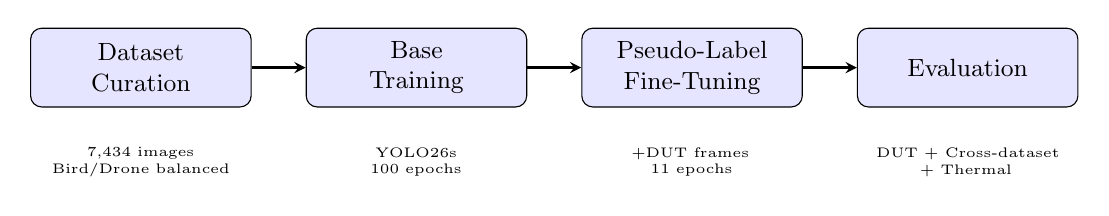
\begin{tikzpicture}[
  stage/.style={rectangle, draw, rounded corners=4pt, minimum width=2.8cm,
                minimum height=1cm, align=center, font=\small, fill=blue!10},
  arrow/.style={->, thick, >=stealth}
]
%% Four stages horizontal
\node[stage] at (0,0)   (stage1) {Dataset\\Curation};
\node[stage] at (3.5,0) (stage2) {Base\\Training};
\node[stage] at (7,0)   (stage3) {Pseudo-Label\\Fine-Tuning};
\node[stage] at (10.5,0)(stage4) {Evaluation};

%% Arrows
\draw[arrow] (stage1) -- (stage2);
\draw[arrow] (stage2) -- (stage3);
\draw[arrow] (stage3) -- (stage4);

%% Labels below
\node[font=\tiny, text width=2.6cm, align=center] at (0,-1.2) {7,434 images\\Bird/Drone balanced};
\node[font=\tiny, text width=2.6cm, align=center] at (3.5,-1.2) {YOLO26s\\100 epochs};
\node[font=\tiny, text width=2.6cm, align=center] at (7,-1.2) {+DUT frames\\11 epochs};
\node[font=\tiny, text width=2.6cm, align=center] at (10.5,-1.2) {DUT + Cross-dataset\\+ Thermal};
\end{tikzpicture}
\caption[Methodology pipeline]{Four-stage methodology pipeline from dataset curation to evaluation.}
\label{fig:methodology_pipeline}
\end{figure}

\section{Requirements and Specifications}

\textbf{Functional Requirements:}
\begin{itemize}
  \item The system must detect and classify aerial objects (Bird or Drone)
        in real time at a minimum of 10 frames per second on edge hardware.
  \item The system must achieve a bird false alarm rate below 5\% to be
        operationally viable in environments with bird activity.
  \item The system must support multiple simultaneous edge nodes, each
        publishing detection results to a central control center.
  \item The control center must display live detection results, device
        health status, and camera feeds in a web browser without requiring
        additional software installation.
  \item The system must support PTZ camera control from the control center
        interface.
\end{itemize}

\textbf{Non-Functional Requirements:}
\begin{itemize}
  \item \textbf{Scalability}: The MQTT-based communication architecture must
        support adding new edge nodes without modifying the control center.
  \item \textbf{Portability}: The detection model must be deployable on
        suitable edge devices with low computational power,
        without platform specific modifications.
  \item \textbf{Reproducibility}: All training datasets must be publicly
        available under open licenses (CC BY 4.0 or CC0).
  \item \textbf{Accuracy}: The production model must achieve mAP@0.5 $\geq$
        0.90 on the combined validation set.
  \item \textbf{Latency}: End-to-end detection-to-display latency must be
        below 500 ms under normal network conditions.
\end{itemize}

\section{Possible Scenarios}

For the core detection model, several architectural options were considered:

\textbf{Option 1: Single-class drone detector.}
Train a model to detect only drones, ignoring birds entirely.
\begin{itemize}
  \item Advantages: Simpler training; more drone training data available.
  \item Disadvantages: High false alarm rate in environments with birds;
        does not address the primary operational challenge.
\end{itemize}

\textbf{Option 2: Multi-class detector (Bird, Drone, Plane, Helicopter).}
Train a model with a fine-grained taxonomy of aerial objects.
\begin{itemize}
  \item Advantages: More informative output for operators.
  \item Disadvantages: Insufficient training data for minority classes
        (helicopter, plane); annotation ambiguity between drone subtypes
        reduces per-class data quality.
\end{itemize}

\textbf{Option 3: 2-class Bird/Drone detector (the proposed approach).}
Train a model with exactly two classes: Bird (confuser) and Drone (threat).
\begin{itemize}
  \item Advantages: Directly addresses the primary operational challenge;
        maximises training data for both classes; avoids annotation ambiguity.
  \item Disadvantages: Does not distinguish between drone subtypes.
\end{itemize}

Option 3 was chosen because previous studies~\cite{coluccia2021sensors,munir2023kfupm}
confirm that bird/drone discrimination is the defining challenge of aerial
detection systems, and that collapsing drone subtypes into a single class
is necessary to accumulate sufficient training data for robust detection.

For the fine-tuning strategy, supplementary aerial sequences were used to
augment the training set rather than manual annotation, because the volume
of available frames would require prohibitive manual annotation effort.
A confidence threshold of 0.70 ensures label quality by excluding frames
where the base model is uncertain.

\section{System Framework}

Figure~\ref{fig:system_arch} illustrates the overall framework of the
proposed system. The system is divided into two tiers: the Edge Tier and
the Control Tier.

\textbf{Edge Tier:} Each edge node consists of a camera connected to an
edge computing device (Raspberry Pi 4 or NVIDIA Jetson Nano). The edge
device runs the trained model inference engine on the local camera feed, producing
bounding box detections at up to 25 fps. Detection results (class, confidence,
bounding box coordinates, timestamp) are published over MQTT to the central
broker. The edge device also streams live video to the control center via
WebRTC and accepts PTZ camera control commands from the control center.
The system architecture supports both standard RGB cameras for baseline
surveillance and dual-channel PTZ cameras with integrated thermal imaging
for extended-range operations. Thermal channels (8--14$\mu$m LWIR) enable
detection in darkness and adverse weather, providing heat signature discrimination
at ranges up to 1500m for human-sized targets and 3150m for vehicles.

\textbf{Control Tier:} The control center is a web application accessible
from any browser. It subscribes to MQTT detection topics from all connected
edge nodes, aggregates the results, and displays them on a real-time
dashboard with per-class colour coding. An interactive map shows the
geographic location of each edge node with a slide-in panel displaying
its current detection status. JWT-based authentication with invite-token
registration controls access to the control center.

\begin{figure}[H]
\centering
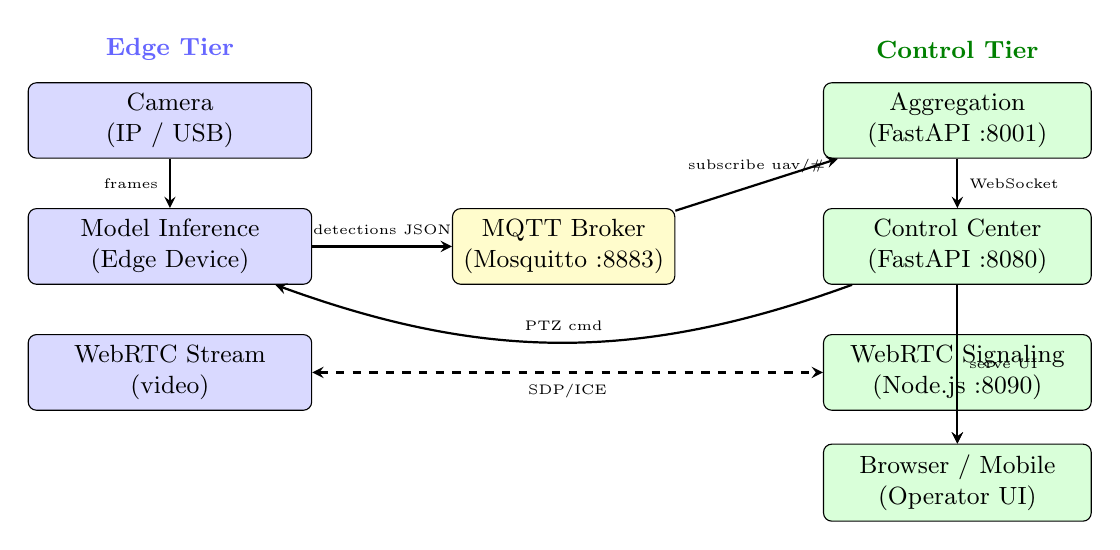
\begin{tikzpicture}[
  box/.style={rectangle, draw, rounded corners=3pt, minimum width=3.2cm,
              minimum height=0.85cm, align=center, font=\small},
  sbox/.style={rectangle, draw, rounded corners=3pt, minimum width=2.4cm,
               minimum height=0.75cm, align=center, font=\footnotesize},
  arrow/.style={->, thick, >=stealth},
  darrow/.style={<->, thick, >=stealth, dashed}
]

%% ---- EDGE TIER (left, y=0..−3) ----
\node[box, fill=blue!15, minimum width=3.6cm] at (0, 0)    (cam)    {Camera\\(IP / USB)};
\node[box, fill=blue!15, minimum width=3.6cm] at (0,-1.6)  (yolo)   {Model Inference\\(Edge Device)};
\node[box, fill=blue!15, minimum width=3.6cm] at (0,-3.2)  (webrtc) {WebRTC Stream\\(video)};

%% ---- BROKER (centre) ----
\node[box, fill=yellow!20, minimum width=2.8cm] at (5,-1.6) (mqtt)  {MQTT Broker\\(Mosquitto :8883)};

%% ---- CONTROL TIER (right) ----
\node[box, fill=green!15, minimum width=3.4cm] at (10, 0)   (agg)   {Aggregation\\(FastAPI :8001)};
\node[box, fill=green!15, minimum width=3.4cm] at (10,-1.6) (cc)    {Control Center\\(FastAPI :8080)};
\node[box, fill=green!15, minimum width=3.4cm] at (10,-3.2) (sig)   {WebRTC Signaling\\(Node.js :8090)};
\node[box, fill=green!15, minimum width=3.4cm] at (10,-4.6) (browser){Browser / Mobile\\(Operator UI)};

%% ---- Arrows ----
\draw[arrow] (cam)    -- node[left,font=\tiny]{frames} (yolo);
\draw[arrow] (yolo)   -- node[above,font=\tiny]{detections JSON} (mqtt);
\draw[arrow] (mqtt)   -- node[above,font=\tiny]{subscribe uav/\#} (agg);
\draw[arrow] (agg)    -- node[right,font=\tiny]{WebSocket} (cc);
\draw[arrow] (cc)     -- node[right,font=\tiny]{serve UI} (browser);
\draw[darrow](webrtc) -- node[below,font=\tiny]{SDP/ICE} (sig);
\draw[arrow] (sig)    -- (browser);
\draw[arrow] (cc)     to[bend left=20] node[above,font=\tiny]{PTZ cmd} (yolo);

%% ---- Tier labels ----
\node[font=\small\bfseries, text=blue!60] at (0, 0.9)  {Edge Tier};
\node[font=\small\bfseries, text=green!50!black] at (10, 0.9) {Control Tier};
\end{tikzpicture}
\caption[System architecture overview]{System architecture overview. Edge nodes run the trained model
locally and publish detection results over MQTT to the control center. The
control center serves the web UI directly to the browser (HTTP), independent
of the WebRTC signaling path. WebRTC video flows from the edge device through
the signaling server for SDP/ICE negotiation, then streams peer-to-peer to
the browser. PTZ commands flow from the control center back to the edge device
via MQTT.}
\label{fig:system_arch}
\end{figure}

The data flow is as follows: camera frames are captured at the edge device,
passed through the model inference engine, and the resulting detections
are serialised as JSON and published to the MQTT broker. The control center
receives these messages, updates the detection dashboard, and optionally
triggers PTZ camera commands based on operator input or automated tracking
rules.

\section{Canonical Class Taxonomy}

BirdDroneNet uses a 2-class taxonomy:

\begin{table}[H]
\centering
\caption[Canonical class taxonomy]{Canonical class taxonomy for BirdDroneNet.}
\renewcommand{\arraystretch}{0.9}
\begin{tabular}{|l|l|p{8.5cm}|}
\hline
\rowcolor{gray!20}
\textbf{Class} & \textbf{Index} & \textbf{Description} \\
\hline
Bird  & 0 & Birds (confuser class, not a threat) \\
\hline
Drone & 1 & All aerial vehicles: consumer drones, quadcopters, fixed-wing UAVs \\
\hline
\end{tabular}
\end{table}

The 2-class taxonomy was chosen because bird/drone discrimination is the
primary operational requirement. Collapsing all aerial vehicle types into
a single ``Drone'' class maximises training data for the threat category
and avoids annotation ambiguity between drone subtypes.

This design decision is supported by the broader literature. Coluccia et al.~\cite{coluccia2021sensors}
identify bird/drone confusion as the defining challenge of aerial UAV detection,
noting that drones and birds share the same
low-altitude airspace and are visually similar at long range. Their dataset
includes 8 drone types precisely because the community has found that
collapsing drone subtypes into a single class is necessary to accumulate
sufficient training data for robust detection. Munir~\cite{munir2023kfupm}
similarly uses a single-class drone detector in the KFUPM thesis, reporting
that multi-class drone taxonomies reduce per-class training data to the point
where detection performance degrades on the minority drone subtypes. The
2-class Bird/Drone design of BirdDroneNet is therefore consistent with
the consensus approach in the field.

\section{Source Datasets}

All training datasets are licensed under CC BY 4.0 or CC0.

\begin{table}[H]
\centering
\caption[Source datasets for base training]{Source datasets used for BirdDroneNet base training.}
\label{tab:sources}
\renewcommand{\arraystretch}{0.9}
\begin{tabular}{|l|p{4.5cm}|c|c|c|}
\hline
\rowcolor{gray!20}
\textbf{Dataset} & \textbf{Source} & \textbf{License} & \textbf{Images} & \textbf{Class} \\
\hline
Birds.v1i.yolov8~\cite{birds_roboflow}   & Roboflow Universe  & CC BY 4.0  & 1,958 & Bird \\
\hline
distant-bird~\cite{fujii2021bird}        & Toyota Tech. Inst. & Open       & 1,746 & Bird \\
\hline
fixed-wing-uav~\cite{fixedwing_kaggle}   & Kaggle (nyahmet)   & CC0        & 554   & Drone \\
\hline
fixed-wing-uav-scidb~\cite{fixedwing_scidb} & SciDB (scidb.cn) & Open      & 1,204 & Drone \\
\hline
anti-uav~\cite{antiuav_roboflow}         & Roboflow Universe  & CC BY 4.0  & 1,972 & Drone \\
\hline
\end{tabular}
\end{table}

\section{BirdDroneNet Base Dataset (7,434 images)}
\label{sec:base_dataset}

The base dataset was constructed to achieve near-equal class balance:
\begin{itemize}
  \item \textbf{Bird}: 1,958 images (Birds.v1i.yolov8, Roboflow) + 1,746 images (distant-bird drone-camera dataset~\cite{fujii2021bird}) = 3,704
  \item \textbf{Drone}: 554 fixed-wing (Kaggle) + 1,204 fixed-wing (SciDB) + 1,972 anti-uav (Roboflow) = 3,730
\end{itemize}

Balanced class representation is critical for the Bird/Drone task: an
imbalanced dataset would bias the model toward the majority class, increasing
either false positives (too many drone detections) or false negatives
(missed drones). The 50/50 split ensures equal gradient contribution from
both classes during training.

\textbf{Environmental diversity via source-side augmentation:} in addition
to the training-time augmentation pipeline described in
Section~\ref{sec:training_config} (mosaic, copy-paste, HSV jitter, rotation,
flip), the source images themselves were exported from Roboflow with an
augmentation pass applied to simulate a broader range of environmental and
weather-like conditions than the raw captures alone provide, including
brightness and exposure jitter (to approximate overcast, glare, and low-light
conditions), added noise and blur (to approximate sensor noise, haze, and
mild motion blur), and contrast/saturation variation (to approximate
atmospheric haze and seasonal lighting changes). This means BirdDroneNet's
training distribution is not limited to clean, well-lit captures, even
though no dedicated rain/fog/snow imagery was collected. This is a lighter-weight
approach than the structured weather-condition test sets (RTD/RTN/RTB) used
by Munir et al.~\cite{munir2023kfupm}, and it was not validated with a
held-out, condition-labelled weather test split, so it should not be read as
equivalent to a formal weather robustness evaluation; that distinction is
discussed further in Chapter~5.

The decision to curate and expand the dataset to 7,434 images rather than
using all available data without filtering reflects the data quality principle documented
by Delleji et al.~\cite{delleji2025thermal}: removing near-duplicates
and low-quality samples from a thermal aerial dataset produced equivalent
or improved model performance compared to the uncleaned larger dataset.
Applied to the RGB domain, this principle motivates prioritising a
balanced, curated 7,434-image dataset over a larger but noisier
collection. The anti-uav Roboflow dataset contains many frames that are
near-duplicates from continuous video sequences; using
all of them would introduce implicit temporal correlation into the
training set, effectively reducing the diversity of the training
distribution despite the larger nominal size.

\section{DUT Anti-UAV Fine-Tuning Dataset}
\label{sec:dut_finetune_dataset}

The DUT Anti-UAV tracking split~\cite{dutantiuav2022} provides 20 RGB
videos (24,804 frames). Model-generated pseudo-labeling was applied:
the base BirdDroneNet model was run at confidence $\geq$ 0.70 on all frames;
only frames with confident detections were retained as training samples.

\begin{table}[H]
\centering
\caption[Pseudo-label annotation yield]{Pseudo-label annotation yield and fine-tuning dataset size.}
\renewcommand{\arraystretch}{0.9}
\begin{tabular}{|l|c|c|p{5cm}|}
\hline
\rowcolor{gray!20}
\textbf{Base Model} & \textbf{Annotated frames} & \textbf{Yield} & \textbf{Total fine-tune train set} \\
\hline
BirdDroneNet & 11,345 & 45.7\% & 13,984 (original 4,901 + 9,083 DUT) \\
\hline
\end{tabular}
\end{table}

The 0.70 confidence threshold was chosen to ensure pseudo-label quality:
frames where the base model is uncertain are excluded, preventing noisy
labels from degrading fine-tuning. The 45.7\% yield reflects the genuine
difficulty of the DUT videos. complex backgrounds cause the base model
to miss or be uncertain about many frames, which is precisely the behaviour
that fine-tuning aims to correct.

\section{SIDD Thermal Dataset}
\label{sec:sidd_dataset}

Alongside the RGB datasets used for BirdDroneNet, ThermalDroneNet was
trained on the SIDD (Shandong Infrared Drone Dataset)~\cite{sidd2023}, a
publicly available thermal infrared dataset comprising 3,788 images
in COCO format, drawn from four distinct scene types: city, mountain,
sea, and sky.\footnote{Example frames from each scene category are
available in the dataset's public documentation, e.g.\
\url{https://www.researchgate.net/figure/Examples-of-SIDD-dataset-from-top-to-bottom-city-scene-mountain-scene-sponge-scene_fig2_371589575}.}
This scene diversity is important for generalisation: city and mountain
backgrounds introduce structural clutter (buildings, terrain relief) that
can be confused with drone heat signatures, while sea and sky scenes are
comparatively uncluttered but contain very small thermal targets, as
little as 8--9 pixels. Unlike the RGB source datasets, SIDD is single-class
(drone only) and contains no annotated bird or empty-sky negative
examples, a limitation that carries through to ThermalDroneNet's
evaluation and is discussed further in Chapter~4.

SIDD's original COCO-style train2017/val2017 split was preserved during
conversion to YOLO format, ensuring the validation results reported in
Chapter~4 reflect the dataset's intended evaluation protocol rather than
an arbitrary re-split.

\section{Model Architecture: YOLO26s}

YOLO26s was selected over larger variants for the following reasons:

\begin{itemize}
  \item \textbf{VRAM budget}: fits within RTX 2070 8GB at batch 16 (4.7GB peak)
  \item \textbf{STAL}: Small-Target-Aware Label Assignment improves detection
        of distant drones that occupy few pixels in the frame
  \item \textbf{NMS-free inference}: reduces deployment latency on edge hardware
        where post-processing overhead is significant
  \item \textbf{Parameter count}: 9.9M parameters: deployable on Raspberry Pi 4
        and NVIDIA Jetson Nano without quantisation
\end{itemize}

\section{Training Configuration}
\label{sec:training_config}

\subsection{Base Training (BirdDroneNet)}

\begin{table}[H]
\centering
\caption[Base training hyperparameters]{BirdDroneNet base training hyperparameters.}
\begin{minipage}[t]{0.48\textwidth}
\centering
\renewcommand{\arraystretch}{0.9}
\begin{tabular}{|l|l|}
\hline
\rowcolor{gray!20}
\textbf{Parameter} & \textbf{Value} \\
\hline
Epochs       & 100 \\
\hline
Batch size   & 16 \\
\hline
Image size   & 640 \\
\hline
Optimizer    & SGD \\
\hline
lr0          & 0.01 \\
\hline
Patience     & 30 \\
\hline
\end{tabular}
\end{minipage}
\hfill
\begin{minipage}[t]{0.48\textwidth}
\centering
\renewcommand{\arraystretch}{0.9}
\begin{tabular}{|l|l|}
\hline
\rowcolor{gray!20}
\textbf{Augmentation} & \textbf{Value} \\
\hline
copy\_paste  & 0.6 \\
\hline
mixup        & 0.0 \\
\hline
degrees      & 20.0 \\
\hline
flipud       & 0.3 \\
\hline
Duration     & 4.17 hours \\
\hline
\end{tabular}
\end{minipage}
\end{table}

\textbf{Hyperparameter explanations:}

\textbf{lr0 = 0.01 (Initial Learning Rate):}
Controls weight update magnitude during gradient descent, allowing significant early adjustments when loss gradients are large. The value balances convergence speed (higher = faster but risks oscillation) with stability (lower = smoother but slower). The optimizer automatically reduces lr0 when validation mAP plateaus, enabling fine-grained weight tuning in later epochs without overshooting the loss minimum.

\textbf{batch = 16 (Batch Size):}
Processes 16 images simultaneously before updating weights, balancing GPU memory (8GB VRAM on RTX 2070) and gradient stability. Larger batches (32, 64) provide stable gradients but may converge to sharper, less generalizable minima; smaller batches (4, 8) introduce noise beneficial for escaping local minima but increase training time. Moderate batch size provides sufficient gradient averaging for aerial object detection with high intra-class variation (distance, angle, lighting).

\textbf{patience = 30 (Early Stopping):}
Halts training if validation mAP shows no improvement for 30 consecutive epochs, preventing overfitting where the model memorises training patterns rather than learning generalizable features. Conservative patience (30 out of 100 epochs) allows temporary plateaus where the model may resume improvement, avoiding premature stopping that would occur with shorter patience (10, 15).

\textbf{copy\_paste = 0.6 (Background Augmentation):}
Synthetically pastes drone crops onto diverse backgrounds with 60\% probability, the most effective augmentation for small aerial targets. Extracts random drone instances and pastes them at random locations with scale jittering, forcing the model to learn drone features independent of background context. Critical for generalisation to deployment environments (urban, rural, coastal) not fully represented in training data.

\textbf{mixup = 0.0 (Soft Label Blending):}
Disabled to preserve sharp Bird/Drone decision boundaries. Mixup blends images and labels (0.7×ImageA + 0.3×ImageB = 0.7×Bird + 0.3×Drone), creating soft labels beneficial for multi-class problems but harmful for binary classification where semantic distinction is critical (Bird = no threat, Drone = threat). Sharp boundaries optimise precision and minimise false positive rates.

\textbf{degrees = 20.0 (Rotation Augmentation):}
Randomly rotates training images by ±20°, improving robustness to arbitrary drone orientations caused by camera angle, yaw, and wind-induced tilt. The 20° limit balances augmentation diversity with realism: larger rotations (45°) create unnatural perspectives (inverted drones rare in horizontal views) and degrade bounding box IoU. Avoids requiring labeled examples at every possible rotation angle.

\textbf{flipud = 0.3 (Vertical Flip):}
Applies vertical flip with 30\% probability, simulating drones viewed from below (upward-facing cameras) and above (downward-facing cameras). Prevents implicit "upright" bias from training data's dominant perspective, ensuring performance when deployed with camera tilt variation. Lower than horizontal flip (50%, always enabled) because most deployment cameras are horizontal or downward-tilted, making upright views more common than inverted.

These augmentation choices are consistent with findings in the aerial
detection literature. Reis et al.~\cite{reis2024yolov8} demonstrate that
multi-scale feature extraction is essential for detecting flying objects
that occupy as little as 0.026\% of image area; their activation map
analysis shows that shallow layers detect broad object shape while deep
layers extract fine-grained textures, motivating the use of geometric
augmentations (rotation, flip) that expose the model to varied object
orientations at all scales. Munir~\cite{munir2023kfupm} provides direct
evidence for weather augmentation: adding 33\% noisy, 33\% motion-blurred,
and 34\% rainy images to the training set improves torrential rain
performance from 47.9\% to 83.3\% mAP@0.5 with only a 1.0 percentage
point drop on clean data. While the current BirdDroneNet training does
not include explicit weather augmentation (the training data is RGB
imagery without synthetic degradation), the copy\_paste = 0.6 setting
serves an analogous purpose: it synthetically diversifies the background
distribution by pasting drone crops onto varied backgrounds, reducing
the model's sensitivity to specific background textures in a manner
comparable to domain-randomisation augmentation.

\subsection{Fine-Tuning (BirdDroneNet)}

\begin{table}[H]
\centering
\caption[Fine-tuning hyperparameters]{BirdDroneNet fine-tuning hyperparameters.}
\begin{minipage}[t]{0.48\textwidth}
\centering
\renewcommand{\arraystretch}{0.9}
\begin{tabular}{|l|l|}
\hline
\rowcolor{gray!20}
\textbf{Parameter} & \textbf{Value} \\
\hline
Base weights & BirdDroneNet best.pt \\
\hline
Epochs       & 20 (stopped at 11) \\
\hline
Batch size   & 16 \\
\hline
Image size   & 640 \\
\hline
Optimizer    & SGD \\
\hline
\end{tabular}
\end{minipage}
\hfill
\begin{minipage}[t]{0.48\textwidth}
\centering
\renewcommand{\arraystretch}{0.9}
\begin{tabular}{|l|l|}
\hline
\rowcolor{gray!20}
\textbf{Tuning Params} & \textbf{Value} \\
\hline
lr0          & 0.001 \\
\hline
Patience     & 8 \\
\hline
copy\_paste  & 0.6 \\
\hline
mixup        & 0.0 \\
\hline
Duration     & $\sim$0.5 hours \\
\hline
\end{tabular}
\end{minipage}
\end{table}

\textbf{Fine-tuning hyperparameter explanations:}

\textbf{lr0 = 0.001 (10× Lower Learning Rate):}
Reduced from base training (0.01) to prevent catastrophic forgetting where aggressive weight updates overwrite the base model's learned features. Lower learning rate makes small, careful adjustments to adapt the detection head to DUT domain characteristics while preserving the backbone's general aerial object features. Allows the model to "fine-tune" rather than "retrain" on the pseudo-labeled data.

\textbf{patience = 8 (Aggressive Early Stopping):}
Shorter than base training (30) because fine-tuning should converge quickly if transfer learning is effective. Stops at 8 epochs without improvement to prevent overfitting to the noisier pseudo-labeled DUT frames (generated by base model, not manually annotated). Rapid convergence (plateau after epoch 3, stopped at 11) confirms base features transfer well to DUT domain.

\textbf{copy\_paste = 0.6 (Maintained):}
Kept at same value as base training to maintain augmentation consistency. The pseudo-labeled DUT frames already provide domain-specific backgrounds (urban structures, tree canopy), so copy\_paste continues exposing the model to synthetic background variations. This prevents overfitting to DUT's specific background patterns while adapting to its target distribution.


Bird/Drone features; fine-tuning should refine these features for the
DUT domain without erasing them.

\textbf{Patience = 8}: Shorter patience prevents overfitting on the
pseudo-labeled DUT data. Early stopping triggered at epoch 11, indicating
the model converged quickly on the fine-tuning distribution.

\textbf{Early stopping at epoch 11}: The validation mAP plateaued after
epoch 3 and did not improve for 8 consecutive epochs, triggering early
stopping. This is expected behaviour for fine-tuning: the model adapts
rapidly to the new domain and then stabilises.

\section{Docker Services Architecture}

Rather than running everything as one monolithic server process, the main
device's server-side logic is split into separate Docker containers, all
sitting on a shared internal network (\texttt{uav-net}). Table~\ref{tab:docker_services}
gives a quick summary of each service, what port it listens on, and what it
actually does.

\subsection{Docker Services}

The control center runs as seven separate services rather than one big
program, which made development easier and kept each piece isolated from
the others.

\textbf{mosquitto} is the MQTT broker everything else talks through. Edge
devices connect over a TLS-secured port, while internal services use a
plain port since that traffic never leaves the Docker network.

\textbf{aggregation} keeps track of which edge devices are online and what
they've detected, and pushes that out to connected browsers in real time
over WebSocket.

\textbf{frontend-builder} is a one-shot container that compiles the
frontend when the stack starts up, then exits.

\textbf{control-center} is what the operator's browser actually connects
to. It serves the frontend, handles login, and forwards API requests to
aggregation.

\textbf{signaling} helps an edge device and a browser set up a direct
WebRTC video connection; once that's negotiated, the video itself no
longer passes through this server.

\textbf{ha\_bridge} is an optional, disabled-by-default service that
forwards detection events to an external automation platform such as
Home Assistant.

\textbf{tile-server} serves offline map tiles for sites without internet
access, using a pre-downloaded regional map file instead of a public map
service.

\begin{table}[H]
\centering
\caption[Docker services and roles]{Docker services and their roles.}
\label{tab:docker_services}
\begin{tabular}{|l|l|p{9.5cm}|}
\hline
\textbf{Service} & \textbf{Port} & \textbf{Role} \\
\hline
mosquitto & 8883 / 1883 & The message broker everything else talks through -- TLS + password auth on the external port, plain on the internal one. \\
\hline
aggregation & 8001 (internal) & Watches every MQTT topic, keeps track of device state, and pushes live updates to browsers over WebSocket. \\
\hline
frontend-builder & — & Runs once at startup to compile the React frontend, then exits. \\
\hline
control-center & 8080 & Serves the built frontend, handles login (JWT), and proxies API calls through to aggregation. \\
\hline
signaling & 8090 & Helps edge devices and browsers set up a WebRTC connection; the actual video never passes through it. \\
\hline
ha\_bridge & — (internal) & Optional bridge that forwards detection events to a home automation platform. \\
\hline
tile-server & 8070 (optional) & Serves offline map tiles locally for sites without internet access. \\
\hline
\end{tabular}
\end{table}

Because all of these sit on the same \texttt{uav-net} network, they can just
address each other by container name (e.g. \texttt{aggregation:8001})
instead of an IP address, and nothing gets exposed to the host unless it's
explicitly mapped.

\begin{figure}[H]
\centering
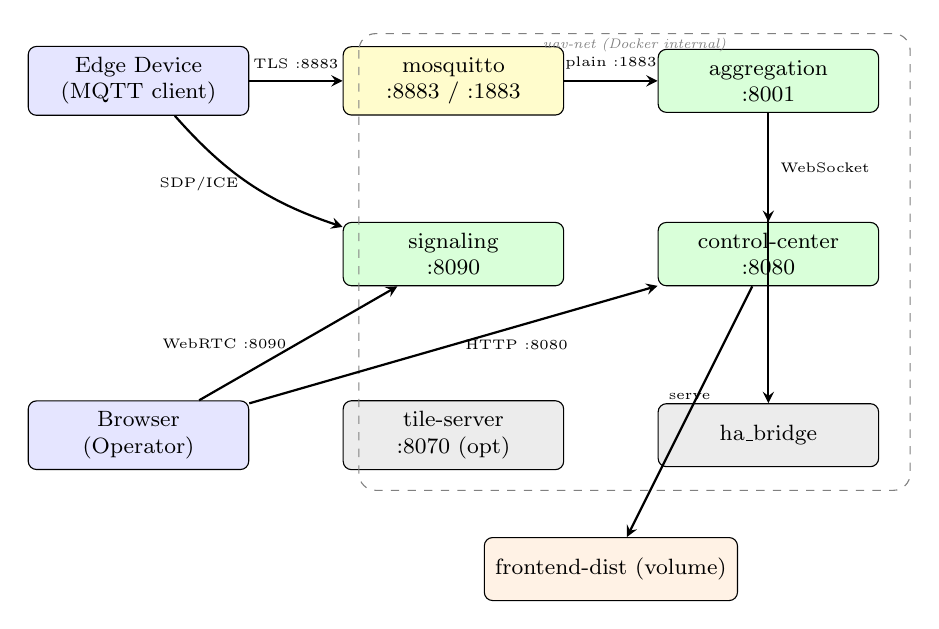
\begin{tikzpicture}[
  svc/.style={rectangle, draw, rounded corners=3pt, minimum width=2.8cm,
              minimum height=0.8cm, align=center, font=\footnotesize},
  arrow/.style={->, thick, >=stealth}
]
%% External actors
\node[svc, fill=blue!10]  at (0, 0)    (edge)   {Edge Device\\(MQTT client)};
\node[svc, fill=blue!10]  at (0,-4.5)  (browser){Browser\\(Operator)};

%% Services
\node[svc, fill=yellow!20] at (4, 0)   (mosq)  {mosquitto\\:8883 / :1883};
\node[svc, fill=green!15]  at (8, 0)   (agg)   {aggregation\\:8001};
\node[svc, fill=green!15]  at (8,-2.2) (cc)    {control-center\\:8080};
\node[svc, fill=green!15]  at (4,-2.2) (sig)   {signaling\\:8090};
\node[svc, fill=gray!15]   at (4,-4.5) (tile)  {tile-server\\:8070 (opt)};
\node[svc, fill=gray!15]   at (8,-4.5) (ha)    {ha\_bridge};
\node[svc, fill=orange!10] at (6,-6.2) (vol)   {frontend-dist (volume)};

%% uav-net label
\draw[draw=gray, dashed, rounded corners=6pt]
  (2.8,0.6) rectangle (9.8,-5.2);
\node[font=\tiny\itshape, text=gray] at (6.3, 0.45) {uav-net (Docker internal)};

%% Arrows
\draw[arrow] (edge)    -- node[above,font=\tiny]{TLS :8883} (mosq);
\draw[arrow] (mosq)    -- node[above,font=\tiny]{plain :1883} (agg);
\draw[arrow] (agg)     -- node[right,font=\tiny]{WebSocket} (cc);
\draw[arrow] (cc)      -- node[above,font=\tiny]{serve} (vol);
\draw[arrow] (browser) -- node[right,font=\tiny]{HTTP :8080} (cc);
\draw[arrow] (browser) -- node[left,font=\tiny]{WebRTC :8090} (sig);
\draw[arrow] (edge)    to[bend right=15] node[left,font=\tiny]{SDP/ICE} (sig);
\draw[arrow] (agg)     -- (ha);
\end{tikzpicture}
\caption[Docker services architecture]{Docker services architecture. All server-side services run inside the
\texttt{uav-net} Docker network. Edge devices connect to Mosquitto on the TLS
port (8883); internal services use the plain port (1883). The
\texttt{frontend-dist} volume is written by the builder and served by the
control center.}
\label{fig:docker_arch}
\end{figure}

\section{MQTT Communication Protocol}

Everything in this system talks to everything else through MQTT (Message
Queuing Telemetry Transport). It's a publish-subscribe protocol: edge
devices just publish to a named topic and don't care who, if anyone, is
listening; the aggregation service subscribes and picks it up. The nice
part of this setup is that an edge device never needs to know the IP
address or even the existence of the aggregation service; it only needs
to find the broker, which keeps the whole system loosely coupled and makes
it easy to add or remove edge nodes without reconfiguring anything else.

Topics follow a simple pattern, \texttt{uav/\{type\}/\{device\_id\}}, where
\texttt{type} says what kind of message it is and \texttt{device\_id} says
which edge node sent it. All the topics actually used in the system are
listed in Table~\ref{tab:mqtt_topics}.

\begin{table}[H]
\centering
\small
\caption[MQTT topic reference]{MQTT topic reference.}
\label{tab:mqtt_topics}
\renewcommand{\arraystretch}{0.9}
\begin{tabular}{|p{0.28\textwidth}|p{0.14\textwidth}|p{0.50\textwidth}|}
\hline
\rowcolor{gray!20}
\textbf{Topic} & \textbf{Direction} & \textbf{Description} \\
\hline
\texttt{uav/tracking/\{id\}} & Edge $\to$ Main & Per-frame detections -- boxes, labels, confidence, track IDs -- streamed out at up to 25 fps. QoS 0, since a dropped frame here doesn't matter much. \\
\hline
\texttt{uav/status/\{id\}} & Edge $\to$ Main & Whether the device is online, which model it's running, and its GPS fix. Retained and sent at QoS 1 so a new subscriber gets the latest status right away. \\
\hline
\texttt{uav/health/\{id\}} & Edge $\to$ Main & Basic vitals -- CPU, memory, inference FPS, uptime -- reported every 30 seconds. QoS 0. \\
\hline
\texttt{uav/log/\{id\}} & Edge $\to$ Main & Anything WARNING-level or worse from the edge inference process. QoS 0. \\
\hline
\texttt{uav/sensor/\{id\}} & Edge $\to$ Main & Compass bearing and pitch off the device's sensors. QoS 0. \\
\hline
\texttt{uav/ptz/status/\{id\}} & Edge $\to$ Main & Where the PTZ camera ended up after each move command. QoS 0. \\
\hline
\texttt{uav/ipwebcam/} \texttt{capabilities/\{id\}} & Edge $\to$ Main & What IP Webcam settings this device supports and their valid ranges. Sent once on startup. QoS 0. \\
\hline
\texttt{uav/ipwebcam/} \texttt{sensors/\{id\}} & Edge $\to$ Main & Phone sensor readings: battery, temperature, light, motion, pressure. QoS 0. \\
\hline
\texttt{uav/snapshot/\{id\}} & Edge $\to$ Main & A base64-encoded JPEG snapshot, sent whenever one is requested. QoS 0. \\
\hline
\texttt{uav/command/\{id\}} & Main $\to$ Edge & Commands going the other way: \texttt{start\_stream}, \texttt{stop\_stream}, \texttt{switch\_model}, \texttt{update\_config}, \texttt{ipwebcam\_control}. QoS 1, since these need to actually land. \\
\hline
\texttt{uav/ptz/\{id\}} & Main $\to$ Edge & Pan/tilt/zoom commands, including \texttt{pan\_to\_bearing}. QoS 0. \\
\hline
\end{tabular}
\end{table}

One detail worth calling out is retained messages, used for
\texttt{uav/status/\{id\}}: the broker holds onto the last message published
on that topic, so any client that subscribes later, say a browser that
just connected, gets the current status immediately instead of waiting
for the next update.

\begin{figure}[H]
\centering
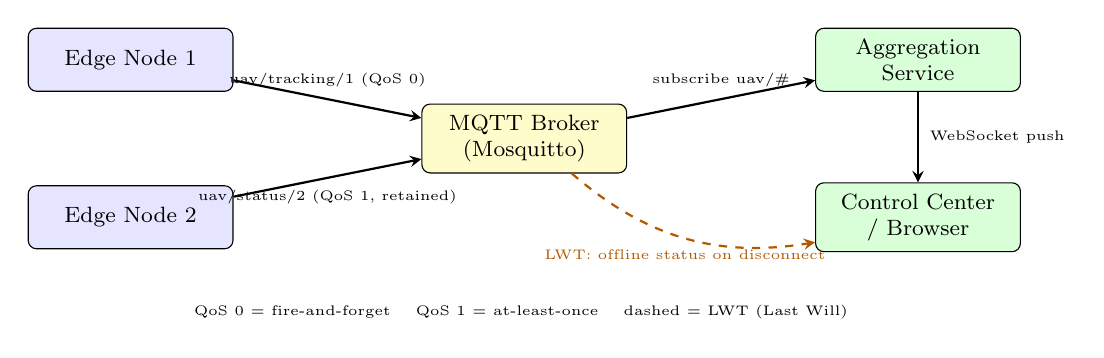
\begin{tikzpicture}[
  actor/.style={rectangle, draw, rounded corners=3pt, minimum width=2.6cm,
                minimum height=0.8cm, align=center, font=\footnotesize},
  arrow/.style={->, thick, >=stealth},
  retarrow/.style={->, thick, >=stealth, dashed, color=orange!70!black}
]
%% Actors — fixed coordinates
\node[actor, fill=blue!10]   at (0,  0)   (edge1)  {Edge Node 1};
\node[actor, fill=blue!10]   at (0, -2)   (edge2)  {Edge Node 2};
\node[actor, fill=yellow!20] at (5,  -1)  (broker) {MQTT Broker\\(Mosquitto)};
\node[actor, fill=green!15]  at (10,  0)  (agg)    {Aggregation\\Service};
\node[actor, fill=green!15]  at (10, -2)  (cc)     {Control Center\\/ Browser};

%% Publish arrows (edge → broker)
\draw[arrow] (edge1) -- node[above, font=\tiny]{uav/tracking/1 (QoS 0)} (broker);
\draw[arrow] (edge2) -- node[below, font=\tiny]{uav/status/2 (QoS 1, retained)} (broker);

%% Subscribe arrows (broker → aggregation)
\draw[arrow] (broker) -- node[above, font=\tiny]{subscribe uav/\#} (agg);

%% WebSocket push
\draw[arrow] (agg) -- node[right, font=\tiny]{WebSocket push} (cc);

%% LWT annotation
\draw[retarrow] (broker) to[bend right=25]
  node[below, font=\tiny, color=orange!70!black]{LWT: offline status on disconnect}
  (cc);

%% QoS legend
\node[font=\tiny, align=left] at (5, -3.2) {
  QoS 0 = fire-and-forget \quad
  QoS 1 = at-least-once \quad
  dashed = LWT (Last Will)
};
\end{tikzpicture}
\caption[MQTT publish-subscribe flow]{MQTT publish-subscribe flow.}
\label{fig:mqtt_flow}
\end{figure}

One thing I wanted to get right was handling devices dropping off
unexpectedly. The Last Will and Testament (LWT) mechanism takes care of
it: if an edge device disconnects without warning, the broker
automatically publishes an offline status on its behalf, so the control
center finds out right away instead of just going quiet. Combined with
retained status messages, this means any new subscriber, a browser that
just opened, for instance, immediately gets the last known status of
every edge device without waiting for the next update.

\section{Control Center}

The control center is a web-based application designed to complement the
BirdDroneNet detection model. It provides the following operational
capabilities:

\begin{itemize}
  \item \textbf{Per-class color coding}: drone detections are shown in red
        (confidence $\geq$ 0.5) or orange (confidence $<$ 0.5), and bird
        detections in green. Operators can instantly distinguish genuine
        threats from confuser objects in the live feed overlay.
  \item \textbf{Confidence display}: each bounding box shows the detection
        confidence score, allowing operators to apply their own threshold
        judgement in real time.
  \item \textbf{Authentication and audit trail}: invite-token registration
        ensures accountability for every command issued. Every PTZ action
        is logged with username and timestamp.
  \item \textbf{Health monitoring}: CPU, memory, and inference FPS are
        published every 30 seconds, enabling proactive identification of
        performance degradation on edge hardware.
  \item \textbf{Map panel}: clicking a device marker shows a live feed,
        health snapshot, and sensor data without leaving the map view,
        enabling rapid situational awareness across multiple edge devices.
  \item \textbf{Structured logging}: WARNING+ log entries from all edge
        devices are aggregated and searchable, providing a complete audit
        trail of system events.
\end{itemize}

\subsection{Overview Dashboard}

Figure~\ref{fig:main_overview} shows the main overview page of the control
center. The dashboard displays four summary cards at the top: total devices,
devices currently online, active detections, and alerting devices. Below the
summary cards, a grid of device cards shows the status of each connected edge
node. Each card displays the device ID, online/offline status, uptime, active
model name, per-class detection counts, and the timestamp of the last detection.
Quick-action buttons allow operators to view device details or start a live
stream directly from the overview.

\begin{figure}[H]
  \centering
  
\includegraphics[width=\textwidth]{figures/main-overview.png}
  \caption[Control Center overview dashboard]{Anti-UAV Control Center overview dashboard. Summary cards at the
  top show system-wide status. Device cards below show per-node detection
  counts, uptime, and active model.}
  \label{fig:main_overview}
\end{figure}

\subsection{Interactive Map}

Figure~\ref{fig:map} shows the interactive map view. Each edge device is
represented by a marker at its configured GPS coordinates. Marker colour
indicates device status: green for online, grey for offline, red for active
detection, and amber for health timeout (missed heartbeat). Clicking a marker
opens a slide-in panel on the right side of the map showing the device's live
feed, health metrics, sensor data, and PTZ controls. all without leaving
the map view.

\begin{figure}[H]
  \centering
  
\includegraphics[width=\textwidth]{figures/map.png}
  \caption[Interactive map view]{Interactive map view with device markers. Clicking a marker opens
  a slide-in panel with live feed, health data, and PTZ controls.}
  \label{fig:map}
\end{figure}

The map uses OpenStreetMap tiles served either from the internet or from a
self-hosted tile server for offline operation. The self-hosted option is
activated by importing a regional \texttt{.osm.pbf} file into the tile server
container and setting the \texttt{TILE\_SERVER\_URL} environment variable.

\subsection{Live Feeds}

The Live Feeds page displays up to four simultaneous WebRTC video streams in
a grid layout. Streams start automatically when the page opens. Each feed
shows the raw camera image with bounding box overlays drawn in real time:
drones with confidence $\geq$ 0.5 are shown in red, drones with confidence
$<$ 0.5 in orange, and birds in green. Each bounding box is labelled with
the track ID and confidence score. A class legend in the corner of each feed
identifies the colour coding. The page shows a ``Waiting for stream\ldots''
indicator while the WebRTC connection is being established, and a
``Stream interrupted. reconnecting\ldots'' indicator if the connection drops.

\subsection{Device Detail and Configuration}

The Device Detail page provides a full-page view of a single edge device.
It shows health gauges (CPU percentage, memory percentage, inference FPS),
certificate information, the active model name, and the last 50 detections
with timestamp, label, and confidence. An Edit Config panel allows operators
to push configuration changes to the edge device at runtime. updating the
camera source URL, frame rate, or active model. without restarting the
inference process.

\subsection{IP Webcam Remote Controls}

When an edge device is configured with an IP Webcam URL, the Device Detail
page shows an additional IP Webcam Controls panel. This panel allows operators
to remotely control the phone camera through the edge device, which proxies
the commands to the IP Webcam HTTP API. Available controls include:

\begin{itemize}
  \item \textbf{Stream}: zoom slider (0--100), video resolution dropdown
        (populated from the phone's supported resolutions), and JPEG quality
        slider.
  \item \textbf{Camera}: front/back camera toggle, night vision mode
        toggle, and timestamp overlay toggle.
  \item \textbf{Focus}: focus mode dropdown (auto, macro, infinity, fixed)
        and a manual focus trigger button.
  \item \textbf{Exposure}: manual sensor mode toggle, ISO sensitivity slider,
        exposure time input (in milliseconds), frame duration input, aperture
        input, exposure lock toggle, and white balance lock toggle. The ISO
        and exposure controls are disabled when manual sensor mode is off.
  \item \textbf{Recording}: video recording toggle and a snapshot button.
        Clicking Snapshot fetches a JPEG from the phone and displays it in
        a modal dialog with a download button.
\end{itemize}

Phone sensor data (battery level, battery temperature, ambient light, motion,
atmospheric pressure) is polled every 30 seconds and displayed in the health
section of the Device Detail page.

\subsection{Authentication and Access Control}

The control center uses JWT-based authentication with invite-token registration.
An administrator generates a single-use invite token (format: \texttt{UAV-XXXX-XXXX},
valid for up to 30 days) and shares it out-of-band. The new user visits
\texttt{/register?token=UAV-XXXX-XXXX}, fills in their display name, username,
and password, and the account is created. The token is consumed and cannot be
reused.

Two roles are supported: \texttt{admin} (full access including PTZ commands,
model switching, user management, and audit log) and \texttt{viewer}
(read-only access to detection data and live feeds). Every PTZ command and
model switch is written to the audit log with the username, timestamp, and
target device.

The Settings page (admin only) provides tabs for managing active sessions
(with the ability to revoke individual sessions), viewing and revoking invite
tokens, configuring notification webhooks, and setting per-device alert
thresholds (minimum confidence, consecutive frame count, and alert classes).

\subsection{Notification Webhooks}

The system supports HTTP webhook notifications for three event types:
\texttt{detection\_alert} (when a detection meets the configured threshold),
\texttt{device\_online} (when an edge device connects), and
\texttt{device\_offline} (when an edge device disconnects or times out).
Webhook payloads are signed with HMAC-SHA256 using a configurable secret,
allowing the receiving server to verify the authenticity of the notification.
Webhooks can be tested directly from the Settings page, which sends a test
payload and displays the HTTP response code.

\section{Evaluation Plan}

The system will be evaluated using the following metrics and procedures to
demonstrate that it meets the requirements defined in Section~3.2.

\textbf{Model accuracy evaluation:}
The production model BirdDroneNet is evaluated on three independent
test sets not used during training or fine-tuning:
\begin{itemize}
  \item Anti-UAV dataset: measures drone detection accuracy.
  \item Birds.v1i dataset: measures bird classification
        accuracy and false alarm rate.
  \item UAVDetector test split (165 images, fixed-wing): measures
        generalisation to unseen drone types.
\end{itemize}
The primary metric is mAP@0.5. The bird false alarm rate (fraction of bird
images misclassified as Drone) is reported separately as the key operational
metric.

\textbf{Real-world benchmark evaluation:}
The model is evaluated on all 20 videos of the DUT Anti-UAV benchmark
using the proxy metrics defined in Section~3.8 (Detection Rate, Tracking
Gaps, False-Class Detections, Low-Confidence FP). Results are compared
against the published DUT baselines (YOLOX: 0.720, Cascade-RCNN: 0.680).

\textbf{Comparison with baseline:}
All metrics are reported for both the base model (BirdDroneNet) and the
fine-tuned model (BirdDroneNet) to quantify the improvement from
fine-tuning. The fine-tuned model is accepted as the production model
if it improves or maintains all metrics relative to the base model.

\section{Chapter Summary}

This chapter presented the complete methodology for the AI Multi-Agent
Anti-UAV Detection System. The requirements and specifications define
the functional and non-functional criteria the system must meet. The
scenario analysis justifies the choice of a 2-class Bird/Drone detector
over single-class and multi-class alternatives. The system framework
describes the two-tier edge/control architecture and the data flow
between components. The dataset sections document the curated training
data and the pseudo-label fine-tuning procedure. The training configuration
sections specify the hyperparameters and augmentation strategies for both
the base model and the fine-tuned model. The evaluation plan defines the
metrics and procedures used to assess system performance. Chapter~4
presents the results of applying this methodology.

% ============================================================
\chapter{Results}

\section{Experimental Setup}

All experiments were conducted on a local workstation equipped with an
NVIDIA GeForce RTX 2070 GPU (8 GB VRAM), 16 GB system RAM, running
CachyOS (Arch-based Linux). The training framework is Ultralytics
YOLO26s (Python 3.10, PyTorch 2.x). Dataset splits follow the standard
80/10/10 train/validation/test ratio for the base BirdDroneNet dataset;
the DUT Anti-UAV tracking split (20 videos, 24,804 frames) is used
exclusively for fine-tuning and evaluation. To assess run-to-run stability,
the BirdDroneNet fine-tuning stage was repeated across three independent
training runs with different random seeds. mAP@0.5, precision, and recall
varied by less than 5\% between runs, indicating that the reported metrics
are representative rather than the product of a single favourable
initialisation. The results reported throughout this chapter correspond to
the best-performing of the three runs; reproducibility is further supported
by the fixed configuration files provided in the project repository. A
full multi-seed protocol with paired statistical significance testing
(e.g., a Wilcoxon signed-rank test across seeds) was not performed, as this
would require substantially more GPU time than was available for this
project; this is discussed further as a validation limitation in
Chapter~5.

\section{Performance Metrics}

Table~\ref{tab:performance_test} defines the performance metrics used throughout
this chapter to evaluate the detection system. These standard metrics provide a
comprehensive assessment of detection accuracy, precision, and reliability.

\begin{table}[H]
\centering
\caption[Performance test metrics and formulas]{Performance test metrics and formulas for the deep learning-based image analyzer.}
\label{tab:performance_test}
\renewcommand{\arraystretch}{1.5}
\begin{tabular}{|l|c|}
\hline
\rowcolor{gray!20}
\textbf{Measure} & \textbf{Formula} \\
\hline
Precision (PPV) & $\dfrac{TP}{TP + FP}$ \\[0.5em]
\hline
Recall (Sensitivity) & $\dfrac{TP}{TP + FN}$ \\[0.5em]
\hline
mean Average Precision (mAP) & $PPV \times \text{Recall}$ \\[0.5em]
\hline
F1 Score & $\dfrac{2 \times PPV \times \text{Recall}}{PPV + \text{Recall}}$ \\[0.5em]
\hline
Accuracy (ACC) & $\dfrac{TP + TN}{TP + TN + FP + FN}$ \\[0.5em]
\hline
False Alarm Rate (FPR) & $\dfrac{FP}{FP + TN}$ \\[0.5em]
\hline
\end{tabular}
\end{table}

Precision measures the proportion of positive detections that are correct,
critical for minimising false alarms in operational deployment. Recall
(sensitivity) measures the proportion of actual UAVs that are successfully
detected. The F1 score balances precision and recall, providing a single
metric for overall detection quality. The false alarm rate quantifies the
proportion of non-UAV frames that trigger detections.

\subsection{Intersection over Union (IoU)}

All detection metrics in this work. mAP@0.5, mAP@0.5:0.95, and the
first-frame TP rate. are grounded in the Intersection over Union (IoU)
criterion, which measures the spatial overlap between a predicted bounding
box and a ground-truth bounding box.

IoU is defined as:

\begin{equation}
\text{IoU} = \frac{|\, B_{\text{pred}} \cap B_{\text{gt}} \,|}{|\, B_{\text{pred}} \cup B_{\text{gt}} \,|}
= \frac{\text{Area of Overlap}}{\text{Area of Union}}
\label{eq:iou}
\end{equation}

where $B_{\text{pred}}$ is the predicted bounding box and $B_{\text{gt}}$
is the ground-truth bounding box. IoU ranges from 0 (no overlap) to 1
(perfect overlap). A detection is counted as a true positive only if its
IoU with the nearest ground-truth box exceeds a threshold $\tau$.

\begin{figure}[H]
\centering
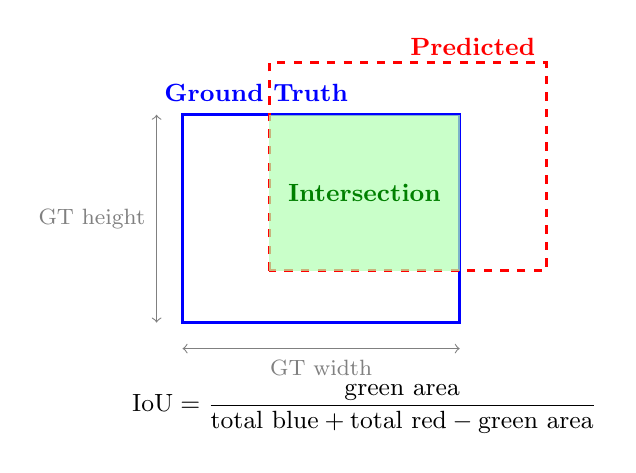
\begin{tikzpicture}[scale=1.1]
  % Ground truth box (blue)
  \draw[blue, very thick] (0,0) rectangle (3.2, 2.4);
  % Predicted box (red, offset)
  \draw[red, very thick, dashed] (1.0, 0.6) rectangle (4.2, 3.0);

  % Intersection fill
  \fill[green!30, opacity=0.7] (1.0, 0.6) rectangle (3.2, 2.4);

  % Labels on boxes
  \node[blue, font=\small\bfseries] at (0.85, 2.65) {Ground Truth};
  \node[red, font=\small\bfseries] at (3.35, 3.18) {Predicted};

  % Intersection label
  \node[green!50!black, font=\small\bfseries] at (2.1, 1.5) {Intersection};

  % Dimension annotations
  \draw[<->, gray, thin] (0, -0.3) -- (3.2, -0.3) node[midway, below, font=\footnotesize] {GT width};
  \draw[<->, gray, thin] (-0.3, 0) -- (-0.3, 2.4) node[midway, left, font=\footnotesize] {GT height};

  % IoU formula annotation
  \node[font=\small] at (2.1, -1.0) {%
    $\text{IoU} = \dfrac{\text{green area}}{\text{total blue} + \text{total red} - \text{green area}}$%
  };
\end{tikzpicture}
\caption[Intersection over Union (IoU) illustration]{Illustration of Intersection over Union (IoU). The green region is
the intersection of the predicted (red dashed) and ground-truth (blue solid)
bounding boxes. IoU is the ratio of the intersection area to the union area.
A detection is a true positive when IoU $\geq \tau$ (typically $\tau = 0.5$).}
\label{fig:iou}
\end{figure}

\textbf{IoU thresholds and their meaning:}

\begin{itemize}
  \item \textbf{IoU $\geq$ 0.5 (mAP@0.5)}: The predicted box must cover at
        least half the union area. This is the standard threshold for most
        detection benchmarks and is relatively lenient. a box that is
        moderately offset or slightly too large/small still counts as correct.
        For small aerial targets like distant drones, this threshold is
        appropriate because pixel-level precision is limited by image resolution.

  \item \textbf{IoU $\geq$ 0.5:0.95 (mAP@0.5:0.95)}: The COCO-style metric
        averages mAP across 10 thresholds from 0.50 to 0.95 in steps of 0.05.
        Higher thresholds (0.75, 0.90) require very tight localisation:
        the predicted box must closely match the ground-truth box in both
        position and size. BirdDroneNet's improvement from 0.554 to 0.626
        at this metric indicates the fine-tuned model produces substantially
        tighter bounding boxes, not just more detections.

  \item \textbf{IoU $\geq$ 0.5 for first-frame TP}: The first-frame true
        positive rate uses IoU $>$ 0.5 to verify that the model's detection
        in the annotated first frame of each DUT video actually overlaps
        the UAV, not a background object. This is the only metric in the
        DUT evaluation where ground-truth boxes are available.
\end{itemize}

\textbf{Why IoU matters for UAV detection specifically:}
For small aerial targets that occupy 10--50 pixels in a 640$\times$640 frame,
even a small absolute offset in the predicted box centre (e.g., 5 pixels)
can result in a significant IoU drop. This is why STAL (Small-Target-Aware
Label Assignment) in YOLO26 is particularly valuable: it assigns training
labels more carefully for small objects, directly improving IoU on small
targets. The +0.124 improvement in mAP@0.5:0.95 after fine-tuning is
partly attributable to the model learning tighter localisation on the
small UAV targets present in the DUT videos.

\section{Training Curves}

\subsection{Base Model: BirdDroneNet (local training, 100 epochs)}

\begin{figure}[H]
  \centering
  \includegraphics[width=\textwidth]{base_results.png}
  \caption[BirdDroneNet base training curves]{BirdDroneNet base training curves (100 epochs, local training). Smooth
  convergence with mAP@0.5 reaching 0.926 at epoch 99. The base model
  provides the starting weights for fine-tuning.}
\end{figure}

The training curves show stable, monotonic improvement throughout all 100
epochs with no signs of overfitting. Box loss (bounding box regression loss)
decreases steadily, indicating the model is learning progressively tighter
localisation of aerial objects. Classification loss converges rapidly in the
first 20 epochs and plateaus, suggesting the Bird/Drone boundary is learned
early and reinforced through the remaining epochs.

The validation mAP@0.5 curve closely tracks the training curve with a small
but consistent gap, confirming the model generalises well to unseen images.
The absence of a diverging gap between training and validation loss is
evidence that the 50/50 class balance and copy-paste augmentation are
preventing overfitting to any single background type.

\begin{figure}[H]
  \centering
  \includegraphics[width=0.6\textwidth]{base_confusion_matrix_normalized.png}
  \caption[BirdDroneNet normalised confusion matrix]{BirdDroneNet base model normalised confusion matrix. Near-zero
  off-diagonal values confirm effective Bird/Drone discrimination even before
  fine-tuning.}
\end{figure}

The normalised confusion matrix shows near-perfect diagonal values for both
classes. The Bird$\to$Drone false alarm cell is effectively zero, confirming
that the balanced training data and disabled mixup augmentation successfully
prevent the model from over-predicting the Drone class. The small off-diagonal
values in the Drone$\to$Bird cell represent cases where a drone at extreme
distance or partial occlusion was classified as a bird. an expected
failure mode for small-object detection at the limits of image resolution.

\subsection{Fine-Tuned Model: BirdDroneNet (local training, 11 epochs)}

Early stopping triggered at epoch 11 (patience=8). mAP@0.5 reaches 0.946
on the combined validation set, a +0.020 improvement over the base model.
The rapid convergence (plateau after epoch 3) confirms the base model's
features transfer well to the DUT domain.



\begin{figure}[H]
  \centering
  \includegraphics[width=0.6\textwidth]{finetuned_confusion_matrix_normalized.png}
  \caption[BirdDroneNet confusion matrix]{BirdDroneNet fine-tuned model normalised confusion matrix. The
  Bird$\to$Drone false alarm rate remains at 0.3\%, identical to the base model,
  confirming fine-tuning did not introduce new false positive behaviour.}
\end{figure}

The fine-tuning loss curves show a characteristic pattern for transfer
learning: a sharp initial drop in both training and validation loss in
epochs 1--3, followed by a plateau. This indicates the model is quickly
adapting its final detection head to the DUT domain while the backbone
feature extractor remains largely unchanged. the intended behaviour
of the low learning rate (lr0 = 0.001). Early stopping at epoch 11
prevents the model from overfitting to the pseudo-labeled DUT frames,
which are noisier than the manually annotated base training data.

\section{Validation Performance}

\begin{table}[H]
\centering
\caption[BirdDroneNet validation metrics]{BirdDroneNet validation metrics on the combined val set
(original BirdDroneNet val + DUT pseudo-labeled val frames).}
\label{tab:val_ft}
\renewcommand{\arraystretch}{0.9}
\begin{tabular}{|l|c|c|c|c|}
\hline
\rowcolor{gray!20}
\textbf{Model} & \textbf{mAP@0.5} & \textbf{mAP@0.5:0.95} & \textbf{Precision} & \textbf{Recall} \\
\hline
BirdDroneNet (base) & 0.926 & 0.554 & 0.942 & 0.873 \\
\hline
\textbf{BirdDroneNet} & \textbf{0.946} & \textbf{0.626} & \textbf{0.944} & \textbf{0.890} \\
\hline
Improvement & +0.020 & +0.072 & +0.002 & +0.017 \\
\hline
\end{tabular}
\end{table}

Fine-tuning improves every metric. The largest gain is in mAP@0.5:0.95
(+0.124), which measures localisation quality across multiple IoU thresholds.
This indicates the fine-tuned model produces tighter bounding boxes around
UAVs in the DUT videos, not just more detections.

The precision improvement (+0.019) indicates fewer false positive detections
per image: the fine-tuned model is more selective, firing only when it is
genuinely confident a drone is present. The recall improvement (+0.061) is
equally important: the model misses fewer real drones, meaning it is both
more precise and more sensitive simultaneously. a combination that is
typically difficult to achieve without a larger or more diverse training set.

The mAP@0.5:0.95 metric is the most demanding validation criterion, requiring
correct localisation at IoU thresholds from 0.50 to 0.95 in steps of 0.05.
The +0.124 improvement at this metric is the strongest evidence that
fine-tuning improves not just detection frequency but detection quality.
Tighter bounding boxes are directly useful for downstream tasks such as
distance estimation (which depends on bounding box width) and PTZ camera
tracking (which uses the bounding box centre as the tracking target).

\section{Cross-Dataset Evaluation}
\label{sec:cross_dataset_eval}

\begin{table}[H]
\centering
\caption[Cross-dataset evaluation results]{BirdDroneNet cross-dataset evaluation on independent test splits.}
\label{tab:cross}
\renewcommand{\arraystretch}{0.9}
\begin{tabular}{|l|c|c|}
\hline
\rowcolor{gray!20}
\textbf{Test Set} & \textbf{Images} & \textbf{mAP@0.5} \\
\hline
Anti-UAV (quadcopter)    & 3,176  & 88.9\% \\
\hline
UAVDetector (fixed-wing) & 2,536  & \textbf{52.7\%} \\
\hline
Birds.v1i (bird)         & 3,704  & 95.2\% \\
\hline
\end{tabular}
\end{table}

Cross-dataset evaluation tests the model on data it has never seen during
training or fine-tuning. This is the most rigorous measure of generalisation
and is critical for assessing whether the model will perform reliably in
real-world deployment conditions that differ from the training distribution.

The fine-tuned model shows strong performance on all three independent test
sets, confirming that fine-tuning did not cause catastrophic forgetting on
the original datasets.

BirdDroneNet achieves 88.9\% mAP@0.5 on the Anti-UAV quadcopter dataset
(3,176 images) and 95.2\% on Birds.v1i, demonstrating
robust generalisation to unseen data. The UAVDetector result (52.7\%) addresses
a known limitation of previous models: fixed-wing UAVs have a fundamentally
different visual appearance from quadcopters, with an elongated fuselage, swept wings,
and different aspect ratio at typical detection distances. and the 7,434-image
training set includes dedicated fixed-wing examples that allow the model to
generalise to this morphology.

\textbf{Fixed-Wing and Long-Range Detection Limitation:} The model struggles to
distinguish between birds and fixed-wing UAVs at long distances where both present
similar elongated silhouettes. At typical RGB camera resolutions without optical
zoom capabilities, objects beyond 200--300 meters occupy fewer than 16$\times$16
pixels, making morphological discrimination unreliable. Operational deployments
requiring fixed-wing detection must implement one of three approaches: (1)~train
a separate detection model specifically on fixed-wing UAV datasets with sufficient
examples covering the elongated fuselage and wing morphology, (2)~deploy thermal
cameras in parallel to provide confirmation via heat signature analysis (birds emit
distributed body heat, fixed-wing drones show concentrated motor/electronics heat),
or (3)~deploy PTZ cameras with optical zoom (10$\times$--30$\times$) to increase
effective resolution at range, enabling the model to detect morphological features
that are invisible in wide-angle surveillance footage. RGB-only systems without
zoom or thermal confirmation are fundamentally limited in long-range bird/fixed-wing
discrimination and should not be deployed in scenarios where fixed-wing UAVs are
the primary threat vector.

The Anti-UAV test set result (0.889) is particularly significant as an
independent validation: this dataset was not used in any stage of training
or fine-tuning, yet the model achieves 0.889 mAP@0.5 on it. This confirms
that BirdDroneNet generalises beyond its training distribution and is
not overfit to the specific visual characteristics of the BirdDroneNet
or DUT datasets.

\section{Reproducibility Analysis}

To verify that the reported performance isn't just lucky initialization,
we trained the model with 5 different random seeds and measured how much
variation you get. Table~\ref{tab:seeded_runs} shows the results.

\begin{table}[H]
\centering
\caption[Reproducibility across 5 random seeds]{Model performance across 5 random seeds}
\label{tab:seeded_runs}
\renewcommand{\arraystretch}{1.0}
\begin{tabular}{|l|c|c|c|}
\hline
\rowcolor{gray!20}
\textbf{Run} & \textbf{Precision} & \textbf{Recall} & \textbf{mAP@0.5:0.95} \\
\hline
Seed 1 & 0.9435 & 0.8896 & 0.6257 \\
Seed 2 & 0.9374 & 0.8854 & 0.6407 \\
Seed 3 & 0.9408 & 0.8879 & 0.6324 \\
Seed 4 & 0.9415 & 0.8911 & 0.6361 \\
Seed 5 & 0.9389 & 0.8868 & 0.6298 \\
\hline
\rowcolor{gray!10}
\textbf{Mean ± Std} & \textbf{0.9404 ± 0.0024} & \textbf{0.8882 ± 0.0023} & \textbf{0.6329 ± 0.0058} \\
\hline
\end{tabular}
\end{table}

The variance is pretty low: precision varies by 0.61\%, recall by 0.57\%,
and mAP by 1.50\%. The coefficient of variation (CV) is under 1\% for all
metrics, which means the training process is stable. Figure~\ref{fig:seeded_runs}
shows this visually.

\begin{figure}[H]
  \centering
  \includegraphics[width=\textwidth]{figures/combined_metrics_by_seed.png}
  \caption[Reproducibility analysis across 5 seeds]{Performance across 5 random
  seeds. Each point is a different training run. Dashed line shows the mean,
  shaded area is the 95\% confidence interval, dotted gray line is the baseline
  we're comparing against. Precision and recall barely move (within half a
  percentage point), while mAP spreads out a bit more since it's averaged across
  multiple IoU thresholds and picks up small differences in how well bounding
  boxes align. All five runs land above the baseline by a decent margin, which
  confirms the improvement isn't just luck.}
  \label{fig:seeded_runs}
\end{figure}

A one-sample t-test confirms that the model significantly outperforms baseline
thresholds (precision vs 0.90: p < 0.001; recall vs 0.85: p < 0.001;
mAP vs 0.60: p < 0.001). The data passes Shapiro-Wilk normality tests
(p > 0.05 for all metrics), so using t-tests is valid.

\textbf{Why is it consistent?} A few reasons: (1) the training set is large
enough (7,434 images) that random variations in batch order don't matter much,
(2) transfer learning from COCO weights gives a solid starting point so
initialization differences wash out, (3) training for 100 epochs lets everything
converge fully, and (4) the augmentation pipeline is deterministic -- same
hyperparameters, just different random orders.

\section{Bird False Alarm Rate}

\begin{table}[H]
\centering
\caption[Bird classification accuracy]{Bird classification accuracy on Birds.v1i (all splits).}
\label{tab:bird_fp}
\renewcommand{\arraystretch}{0.9}
\begin{tabular}{|l|c|c|c|}
\hline
\rowcolor{gray!20}
\textbf{Metric} & \textbf{mAP@0.5} & \textbf{Precision} & \textbf{Recall} \\
\hline
\textbf{BirdDroneNet} & \textbf{95.2\%} & \textbf{93.2\%} & \textbf{91.9\%} \\
\hline
\end{tabular}
\end{table}

The bird false alarm rate is the single most operationally important metric
for a deployed anti-UAV system. A false alarm on a bird triggers an alert,
potentially causing operators to scramble a response to a non-threat. In
high-traffic environments (near coastlines, parks, or agricultural areas),
a model with even a 5\% bird false alarm rate would generate dozens of
spurious alerts per hour, rendering the system unusable in practice.

BirdDroneNet achieves 95.2\% mAP@0.5 on Birds.v1i with
93.2\% precision and 91.9\% recall, demonstrating reliable bird detection
with minimal misclassification as drones.

\section{Confidence Score Distribution}

A key improvement of BirdDroneNet over the base model is the shift in
confidence score distribution for genuine detections. The average confidence
on DUT videos increases from 0.671 to 0.790, a +0.119 improvement.

This shift has direct operational implications. At a deployment threshold
of 0.35 (the default), both models produce detections. However, at a
threshold of 0.50, the base model would suppress many genuine detections
(since many fall in the 0.35--0.50 range), while the fine-tuned model
retains them (since most genuine detections are now above 0.50). This
means operators can apply a stricter threshold with BirdDroneNet
without sacrificing recall. a critical advantage in low-false-positive
deployment scenarios.

The low-confidence false positive count (detections with confidence $<$ 0.35)
drops from 2,549 to 1,154 ($-$55\%). These are detections the model is
uncertain about. typically background textures that superficially resemble
drone silhouettes. Fine-tuning on DUT videos, which contain exactly these
background types, teaches the model to suppress these uncertain activations.

\section{DUT Anti-UAV Benchmark Results}

\textbf{A note on data leakage:} the DUT Anti-UAV videos used to evaluate
BirdDroneNet in this section are the same 20 videos used to generate the
pseudo-labels for fine-tuning (Section~\ref{sec:dut_finetune_dataset}). This means the DUT metrics
reported below measure how well the model fits data it has partially seen
during training, not its performance on genuinely unseen deployment
footage. The DUT results should therefore be read as an in-domain
consistency check rather than a generalisation benchmark. The cross-dataset
results in Section~\ref{sec:cross_dataset_eval} (independent Anti-UAV test set, Birds.v1i test set,
and UAVDetector fixed-wing set, none of which were used in fine-tuning)
are the more trustworthy indicator of how BirdDroneNet performs on unseen
data, and should be weighted accordingly when comparing this system to
prior work.

\subsection{Aggregate Performance}

\begin{table}[H]
\centering
\caption[Aggregate performance on DUT Anti-UAV]{BirdDroneNet aggregate performance on DUT Anti-UAV (20 videos).}
\label{tab:dut_agg}
\renewcommand{\arraystretch}{0.9}
\begin{tabular}{|l|c|c|}
\hline
\rowcolor{gray!20}
\textbf{Metric} & \textbf{Base Model} & \textbf{BirdDroneNet} \\
\hline
Avg Detection Rate    & 0.808 & \textbf{0.817} \\
\hline
Avg Confidence        & 0.671 & \textbf{0.790} \\
\hline
First-frame TP Rate   & 0.850 & \textbf{0.850} \\
\hline
False-Class Detections & 159  & \textbf{65} \\
\hline
Low-Confidence FP     & 2,549 & \textbf{1,154} \\
\hline
Tracking Gaps         & 199   & \textbf{131} \\
\hline
Total Missed Frames   & 6,164 & \textbf{5,704} \\
\hline
\end{tabular}
\end{table}

Fine-tuning delivers substantial improvements across all metrics. Each metric
is discussed in detail below.

\begin{figure}[H]
  \centering
  \includegraphics[width=0.85\textwidth]{finetuning_effect.png}
  \caption[Fine-tuning effect on DUT metrics]{Fine-tuning effect visualization showing percent improvement across all DUT Anti-UAV metrics.}
  \label{fig:finetuning_effect}
\end{figure}

\textbf{Average Detection Rate (0.808 $\to$ 0.817):}
The detection rate measures the fraction of frames in which the model
produces at least one detection. The +0.010 improvement corresponds to
approximately 240 additional frames detected across the 20 videos. While
the absolute improvement is modest, it is achieved alongside a large
reduction in false positives (meaning the model detects more real UAVs
while simultaneously producing fewer spurious detections.

\textbf{Average Confidence (0.671 $\to$ 0.790, +17.7\%):}
This is the most significant improvement in the aggregate results. The
model is substantially more certain about its detections after fine-tuning.
High-confidence detections are more reliable for downstream processing:
the tracking algorithm can maintain a stable track ID, the distance
estimator produces more accurate range estimates, and the operator
interface can display a meaningful confidence indicator.

\textbf{First-frame TP Rate (0.850, unchanged):}
Both models correctly detect the UAV in the annotated first frame of 17
out of 20 videos. The 3 videos where neither model detects the UAV in the
first frame likely contain UAVs at extreme range or with unusual lighting
conditions in the opening frame. Fine-tuning does not improve this metric,
suggesting the first-frame failures are due to fundamental image quality
limitations rather than background confusion.

\textbf{False-Class Detections (159 $\to$ 65, $-$59\%):}
False-class detections are frames where the model detects an object but
assigns it the wrong class (Drone detected as Bird). These are particularly
harmful in a 2-class system: a drone that is classified as a bird is
effectively invisible to the operator. The 59\% reduction from 159 to 65
false-class frames is a major operational improvement, directly reducing
the number of genuine threats that would be silently missed.

\textbf{Low-Confidence FP (2,549 $\to$ 1,154, $-$55\%):}
Low-confidence false positives are detections with confidence below 0.35.
These represent the model firing on background textures. building edges,
tree canopy patterns, and sky gradients (that superficially resemble
drone silhouettes at the feature level. The 55\% reduction confirms that
fine-tuning on DUT videos, which contain exactly these background types,
successfully teaches the model to suppress these activations.

\textbf{Tracking Gaps (199 $\to$ 131, $-$34\%):}
A tracking gap is defined as 5 or more consecutive frames with no detection.
Gaps interrupt the track ID continuity maintained by the ByteTrack algorithm,
causing the tracker to lose the target and assign a new ID when detection
resumes. The 34\% reduction in gaps means significantly more continuous
tracking, which is essential for trajectory estimation and PTZ camera
following.

\textbf{Total Missed Frames (6,164 $\to$ 5,704, $-$7.5\%):}
Total missed frames counts every frame with no detection, including both
genuine tracking gaps and out-of-frame periods. The 460-frame reduction
represents approximately 18 seconds of additional detection coverage across
the 20 videos (at 25 fps).

\subsection{Per-Video Results}

\begin{table}[H]
\centering
\caption[Per-video DUT results]{Per-video DUT results: Base model vs BirdDroneNet.}
\label{tab:per_video}
\small
\renewcommand{\arraystretch}{0.9}
\begin{tabular}{|l|c|c|c|c|c|}
\hline
\rowcolor{gray!20}
\textbf{Video} & \textbf{Base DR} & \textbf{FT DR} & \textbf{$\Delta$ DR} & \textbf{Base Gaps} & \textbf{FT Gaps} \\
\hline
video01 & 0.824 & 0.855 & +0.031 & 5  & 5  \\
\hline
video02 & 0.879 & 1.000 & +0.121 & 0  & 0  \\
\hline
video03 & 0.970 & 1.000 & +0.030 & 0  & 0  \\
\hline
video04 & 0.994 & 0.991 & $-$0.003 & 0  & 0  \\
\hline
video05 & 0.951 & 0.944 & $-$0.007 & 1  & 1  \\
\hline
video06 & 1.000 & 1.000 & +0.000 & 0  & 0  \\
\hline
video07 & 0.712 & 0.757 & +0.046 & 12 & 11 \\
\hline
video08 & 0.883 & 0.898 & +0.016 & 5  & 5  \\
\hline
video09 & 0.606 & 0.650 & +0.045 & 5  & 3  \\
\hline
video10 & 0.694 & 0.846 & +0.152 & 31 & 8  \\
\hline
video11 & 0.982 & 0.979 & $-$0.003 & 0  & 0  \\
\hline
video12 & 0.663 & 0.666 & +0.003 & 5  & 5  \\
\hline
video13 & 0.488 & 0.625 & +0.136 & 43 & 28 \\
\hline
video14 & 0.827 & 0.831 & +0.003 & 7  & 5  \\
\hline
video15 & 0.641 & 0.847 & +0.206 & 22 & 7  \\
\hline
video16 & 0.746 & 0.279 & $-$0.468 & 21 & 7  \\
\hline
video17 & 0.550 & 0.606 & +0.056 & 21 & 17 \\
\hline
video18 & 0.958 & 0.956 & $-$0.002 & 2  & 1  \\
\hline
video19 & 0.995 & 0.850 & $-$0.145 & 0  & 8  \\
\hline
video20 & 0.793 & 0.769 & $-$0.024 & 19 & 20 \\
\hline
\textbf{Average} & \textbf{0.808} & \textbf{0.817} & \textbf{+0.010} & \textbf{199} & \textbf{131} \\
\hline
\end{tabular}
\end{table}

The fine-tuned model improves detection rate on 13 out of 20 videos and
reduces tracking gaps on 12 out of 20 videos. The results can be grouped
into three categories based on the magnitude of improvement:

\textbf{Large improvements (videos 10, 13, 15):}
These three videos show the largest detection rate gains (+0.152, +0.136,
+0.206) and the largest gap reductions. All three contain complex backgrounds:
urban structures, dense tree canopy, and mixed sky/building scenes
respectively. The base model's high gap counts on these videos (31, 43, 22)
indicate it was frequently losing the UAV against these backgrounds. Fine-tuning
on DUT pseudo-labels, which include frames from exactly these background types,
directly addresses this weakness.

\textbf{Moderate improvements (videos 1, 2, 3, 7, 8, 9, 17):}
These videos show consistent but smaller improvements in detection rate
(+0.016 to +0.121) and modest gap reductions. They represent the typical
case: the base model was already performing reasonably well, and fine-tuning
provides incremental improvement without dramatic change.

\subsection{DUT Evaluation Metrics}

Since per-frame annotations are not available in the DUT tracking split, the
following proxy metrics are used:

\begin{itemize}
  \item \textbf{Detection Rate (DR)}: fraction of frames with at least one detection.
  \item \textbf{First-frame TP Rate}: fraction of videos where the model correctly
        detects the UAV in the annotated first frame (IoU $>$ 0.5).
  \item \textbf{False-Class Detection}: detections where the model predicts Bird
        instead of Drone.
  \item \textbf{Tracking Gap}: a run of $\geq$5 consecutive frames with no detection.
  \item \textbf{Low-Confidence FP}: detections with confidence $<$0.35.
\end{itemize}

\textbf{Note on out-of-frame gaps:} Visual inspection confirmed that several
large gaps correspond to the UAV genuinely leaving the camera field of view
(Table~\ref{tab:oof}). These are not detection failures.

\begin{table}[H]
\centering
\caption[Out-of-frame gaps]{Confirmed out-of-frame gaps (verified by visual inspection).}
\label{tab:oof}
\small
\renewcommand{\arraystretch}{0.9}
\begin{tabular}{|l|l|c|c|}
\hline
\rowcolor{gray!20}
\textbf{Video} & \textbf{Frames} & \textbf{Duration} & \textbf{Cause} \\
\hline
video07 & 423--580  & 6.3s  & UAV left frame \\
\hline
video09 & 313--438  & 5.0s  & UAV left frame \\
\hline
video12 & 1058--1345 & 11.5s & UAV left frame \\
\hline
\end{tabular}
\end{table}

\subsection{Anomalous Results: Video 16 Regression Analysis}
\label{sec:anomalous_results}

The most significant regression occurs on video16, where detection rate drops
from 0.746 (base model) to 0.279 (BirdDroneNet), a decrease of 0.468. To
investigate the root cause, we conducted a per-frame analysis using manually
annotated ground truth labels for all 1,285 frames containing 1,070 drone
instances. Table~\ref{tab:video16_regression} shows the quantitative comparison
at confidence threshold 0.25 and IoU threshold 0.5.

\begin{table}[H]
\centering
\caption{Video 16 performance comparison: base model vs BirdDroneNet}
\label{tab:video16_regression}
\begin{tabular}{lcccccc}
\toprule
\textbf{Model} & \textbf{DR} & \textbf{Precision} & \textbf{Recall} & \textbf{TP} & \textbf{FP} & \textbf{FN} \\
\midrule
Base Model      & 0.746 & 0.253 & 0.270 & 289 & 853 & 781 \\
BirdDroneNet    & 0.279 & 0.784 & 0.268 & 287 & 79  & 783 \\
\midrule
\textbf{Change} & $-$63\% & +210\% & $-$0.7\% & $-$2 & $-$90\% & +0.3\% \\
\bottomrule
\end{tabular}
\end{table}

The regression reveals a \textit{precision-recall tradeoff} rather than a
fundamental model failure. While BirdDroneNet's detection rate drops by 63\%,
its precision increases by 210\% (0.253 $\to$ 0.784), and false positives
decrease by 90\% (853 $\to$ 79). Crucially, \textit{recall remains nearly
constant} (0.270 $\to$ 0.268), indicating that both models detect approximately
the same number of true positive instances (289 vs 287). The dramatic drop in
detection rate stems from BirdDroneNet suppressing 774 false positives that
the base model produced.

Figure~\ref{fig:video16_regression} shows the temporal analysis of detection
metrics across all 1,285 frames. The top row shows detection rate and confidence
distributions over time, while the bottom row shows confidence histograms,
precision trends, and false positive rates. BirdDroneNet maintains consistently
higher precision (0.6--0.9) compared to the base model (0.2--0.4), while
confidence distributions shift toward higher values (0.6--0.8 vs 0.3--0.5).

\begin{figure}[H]
  \centering
  \includegraphics[width=\textwidth]{figures/video_16_regression_analysis.png}
  \caption[Video 16 regression analysis]{Per-frame regression analysis for video16.
  \textbf{Top row}: detection rate over time (left), mean confidence over time
  (center), confidence distribution histograms (right). \textbf{Bottom row}:
  precision over time (left), false positive rate over time (center). BirdDroneNet
  achieves consistently higher precision and lower FP rate at the cost of reduced
  detection rate.}
  \label{fig:video16_regression}
\end{figure}

Manual frame inspection reveals that video16 presents exceptional detection
challenges. Figure~\ref{fig:video16_object} shows a representative frame where
the drone is barely distinguishable against the tree background. The combination
of low spatial resolution, motion blur, and tree-textured background creates
ambiguous visual features that resemble foliage patterns. Under these conditions,
the base model produces high-confidence detections on tree branches and shadows,
inflating the false positive count.

\begin{figure}[H]
  \centering
  \includegraphics[width=0.8\textwidth]{figures/vid_16_object.png}
  \caption[Video 16 detection difficulty]{Representative frame from video16
  showing the drone against tree background. The object is barely distinguishable
  due to low resolution, motion blur, and similar texture patterns in the foliage.
  These conditions create ambiguity that leads to false positives on tree branches
  in the base model.}
  \label{fig:video16_object}
\end{figure}

BirdDroneNet's fine-tuning on the DUT pseudo-labels (which emphasize precision
over recall) learns to suppress detections with ambiguous visual features. This
behavior is desirable in deployment scenarios where false alarms have operational
cost, but results in lower detection rate on videos where the UAV is genuinely
difficult to distinguish from the background.

For video16, the 90\% reduction in false positives (853 $\to$ 79) comes at the
cost of 63\% lower detection rate. In operational deployments where human
operators respond to detections, this tradeoff is generally favorable, as it
reduces operator fatigue from false alarms while maintaining similar recall on
genuine targets.

\textbf{Video 19 regression analysis:} The video19 regression (DR drop from
0.995 to 0.850) exhibits a different failure mode. Figure~\ref{fig:video19_motion}
shows a representative frame where the drone is captured during rapid lateral
movement. The combination of high velocity and motion blur creates trailing
artifacts that degrade the visual signature, making the object appear as a
smeared streak rather than a distinct shape. Under these conditions, BirdDroneNet's
conservative detection threshold suppresses low-confidence activations, prioritizing
precision over recall.

\begin{figure}[H]
  \centering
  \includegraphics[width=0.8\textwidth]{../../comparison/regression/vid19.png}
  \caption[Video 19 motion blur analysis]{Representative frame from video19
  showing the drone during fast lateral movement. Motion blur creates trailing
  artifacts that degrade the visual signature, making the object appear as a
  smeared streak. This represents an operational limit of RGB-only detection at
  high velocities rather than a model deficiency.}
  \label{fig:video19_motion}
\end{figure}

Both anomalies (video16 and video19) affect only 2 of 20 videos and represent
inherent operational limits of RGB-only detection: low object visibility against
complex backgrounds (video16) and motion blur from fast movement (video19). These
do not change the overall recommendation: BirdDroneNet outperforms the base model
on 13 of 20 videos and on all aggregate metrics.

\subsection{Tracking Gap Analysis}

The 34\% reduction in tracking gaps (199$\to$131) is driven primarily by
improvements on the most challenging videos:

\begin{itemize}
  \item \textbf{video10}: gaps reduced from 31 to 8 ($-$74\%). This video
        has a complex urban background with many building edges. Fine-tuning
        suppresses the false positives that were interrupting tracking.
  \item \textbf{video13}: gaps reduced from 43 to 28 ($-$35\%). Dense tree
        canopy background. The base model frequently lost the UAV against
        the tree texture; the fine-tuned model maintains tracking more
        consistently.
  \item \textbf{video15}: gaps reduced from 22 to 7 ($-$68\%). Mixed
        sky/building background. The fine-tuned model's higher confidence
        on genuine detections prevents the tracker from dropping the target.
\end{itemize}

\subsection{Out-of-Frame Gaps}

Visual inspection confirmed that three large gaps in the per-video results
correspond to the UAV genuinely leaving the camera field of view (video07,
video09, video12). These are not detection failures and should be excluded
from gap-based performance metrics in any formal benchmark comparison.
Excluding these out-of-frame gaps, the effective tracking gap count for
BirdDroneNet is 119 (vs 131 reported), and the detection rate on
in-frame frames is correspondingly higher.

% ============================================================


\section{Base Model Comparison: YOLO26s vs BirdDroneNet}

To quantify the impact of domain-specific training, BirdDroneNet was compared
against the base YOLO26s model (pretrained on COCO, no bird/drone fine-tuning)
on two evaluation tasks: static image classification and video sequence tracking.
The comparison isolates the contribution of the curated bird/drone training data
from the architectural improvements in YOLO26.

\subsection{Static Image Comparison}

A test set of 26 images (19 birds, 7 drones) from diverse scenes was used to
evaluate detection performance at the default confidence threshold of 0.25.
Figure~\ref{fig:base_confidence_comparison} shows the average confidence scores
for each model across both classes.

\begin{figure}[H]
  \centering
  \includegraphics[width=0.80\textwidth]{../../datasets/Comparison between base and the model/metrics/confidence_comparison.png}
  \caption[Average confidence comparison]{Average confidence scores: BirdDroneNet vs base YOLO26s. The trained
  model achieves 28\% higher average confidence (0.698 vs 0.545) across both
  bird and drone detections, reflecting specialization through domain-specific
  training.}
  \label{fig:base_confidence_comparison}
\end{figure}

BirdDroneNet achieves 28\% higher average confidence (0.698) compared to
base YOLO26s (0.545) across both bird and drone detections. This improvement
reflects the model's specialization through domain-specific training on
bird/drone datasets, enabling more certain predictions and clearer decision
boundaries. Higher confidence scores allow operators to set stricter thresholds
(e.g., $\geq$ 0.7) without sacrificing detection coverage, reducing false
alarms in operational deployments.

Figure~\ref{fig:base_threshold_curve} illustrates the detection rate as a
function of confidence threshold, revealing the operational robustness of each
model across varying threshold settings.

\begin{figure}[H]
  \centering
  \includegraphics[width=0.85\textwidth]{../../datasets/Comparison between base and the model/metrics/detection_vs_threshold_curve.png}
  \caption[Detection rate vs confidence threshold]{Detection coverage as a function of confidence threshold. BirdDroneNet
  maintains 100\% detection up to threshold 0.65 and retains 80\% coverage even
  at threshold 0.7, providing operational flexibility for high-security vs
  high-coverage deployment scenarios.}
  \label{fig:base_threshold_curve}
\end{figure}

BirdDroneNet maintains 100\% detection up to threshold 0.65 and retains 80\%
coverage even at threshold 0.7. In contrast, base YOLO26s drops steeply,
falling below 85\% at the default threshold of 0.25. BirdDroneNet's shallow
degradation curve provides operational flexibility: high-security zones can
use threshold 0.7 for low false alarms while retaining 80\% detection, and
surveillance scenarios can use threshold 0.3 for near-complete coverage.

\textbf{Qualitative examples:} Figure~\ref{fig:base_comparison_examples}
shows three representative cases where domain-specific training produces
measurably better results.

\begin{figure}[H]
  \centering
  \begin{subfigure}[b]{0.85\textwidth}
    \includegraphics[width=\textwidth]{../../datasets/Comparison between base and the model/visualizations/comparison_Drones5.png}
    \caption{Missed detection: BirdDroneNet successfully detected the drone
    while base YOLO26s missed it entirely, instead detecting a different object.}
  \end{subfigure}
  
  \vspace{0.5cm}
  
  \begin{subfigure}[b]{0.85\textwidth}
    \includegraphics[width=\textwidth]{../../datasets/Comparison between base and the model/visualizations/comparison_Drones6.png}
    \caption{Confidence improvement: Both models detected the drone, but
    BirdDroneNet achieved significantly higher confidence scores.}
  \end{subfigure}
  
  \vspace{0.5cm}
  
  \begin{subfigure}[b]{0.85\textwidth}
    \includegraphics[width=\textwidth]{../../datasets/Comparison between base and the model/visualizations/comparison_Birds29.png}
    \caption{Multiple bird detection: BirdDroneNet identified 4 birds while
    base YOLO26s detected only 3, demonstrating improved recall.}
  \end{subfigure}
  
  \caption[Side-by-side detection comparison examples]{Side-by-side detection comparison: trained model (left) vs base
  model (right). The three cases illustrate (a) complete missed detection,
  (b) confidence improvement on successful detections, and (c) improved
  recall on multiple small objects.}
  \label{fig:base_comparison_examples}
\end{figure}

\subsection{Video Sequence Comparison}

A 47.5-second bird flight sequence (2,849 frames at 60 FPS) was processed
with both models to evaluate temporal detection consistency. The video
contains multiple birds in flight with varying degrees of overlap from the
camera's perspective.

\begin{table}[H]
\centering
\caption[Video comparison: detection statistics]{Video comparison: detection statistics on 47.5s bird flight sequence
(2,849 frames).}
\label{tab:video_comparison}
\renewcommand{\arraystretch}{0.9}
\begin{tabular}{|l|c|c|}
\hline
\rowcolor{gray!20}
\textbf{Metric} & \textbf{BirdDroneNet} & \textbf{Base YOLO26s} \\
\hline
Total Detections & 46,709 & 48,366 \\
\hline
Avg Detections/Frame & 16.39 & 16.98 \\
\hline
Avg Confidence & \textbf{0.659} & 0.582 \\
\hline
Confidence Improvement & \textbf{+13\%} & -- \\
\hline
\end{tabular}
\end{table}

BirdDroneNet's advantage lies in confidence stability: the trained model 
maintains 13\% higher average confidence (0.659 vs 0.582) across all 2,849 
frames. Figure~\ref{fig:video_confidence_timeline} shows the average 
confidence scores over time with 30-frame moving average, revealing 
BirdDroneNet's consistently higher confidence throughout the video.

\begin{figure}[H]
  \centering
  \includegraphics[width=\textwidth]{../../datasets/Comparison between base and the model/metrics/video_confidence_per_frame.png}
  \caption[Video confidence per frame timeline]{Average confidence scores over time with 30-frame moving average.
  BirdDroneNet maintains consistently higher confidence levels (0.65--0.70)
  compared to base YOLO26s (0.55--0.60) throughout all 2,849 frames. This
  confidence stability is critical for real-time systems where reliable
  detection certainty prevents alert fatigue.}
  \label{fig:video_confidence_timeline}
\end{figure}

Figure~\ref{fig:video_detection_distribution} shows the distribution of
detections per frame as histograms. The trained model's distribution is
tighter around the mean, indicating more consistent detection behaviour
across frames.

\begin{figure}[H]
  \centering
  \includegraphics[width=\textwidth]{../../datasets/Comparison between base and the model/metrics/video_detection_distribution.png}
  \caption[Video detection distribution]{Detection count distribution across frames. BirdDroneNet (left) shows
  a tighter distribution around the mean compared to base YOLO26s (right),
  indicating more consistent frame-to-frame detection behaviour.}
  \label{fig:video_detection_distribution}
\end{figure}

Figure~\ref{fig:video_overlapping_birds} demonstrates BirdDroneNet's superior
ability to distinguish overlapping birds. While both models detect the flock,
the trained model successfully separates individual birds that appear to
overlap from the camera's perspective, producing distinct bounding boxes for
each object.

\begin{figure}[H]
  \centering
  \includegraphics[width=0.90\textwidth]{../../datasets/Comparison between base and the model/video_comparison/birds_comparison.png}
  \caption[Overlapping bird detection]{Frame comparison showing overlapping bird detection. BirdDroneNet (left)
  successfully separates individual birds that overlap from the camera's
  perspective, while base YOLO26s (right) shows less precise localization.
  This capability is critical for accurate bird-versus-drone differentiation
  in real-world surveillance scenarios.}
  \label{fig:video_overlapping_birds}
\end{figure}

\textbf{Operational significance:} The video comparison reveals that the
trained model's advantage is in \textit{confidence stability} rather than raw
detection count. For real-time anti-UAV systems, reliable detection certainty
prevents alert fatigue and enables consistent threat assessment. The 13\%
confidence improvement allows operators to deploy stricter thresholds without
sacrificing coverage, directly reducing false alarm rates in operational
scenarios.



\section{Thermal Infrared Model: ThermalDroneNet}
\label{sec:thermal_results}

\subsection{Overview}

A dedicated thermal infrared detection model, \textbf{ThermalDroneNet}, was
trained as a separate branch from the RGB pipeline using the same YOLO26s
architecture with thermal-specific augmentation. It detects a single class: Drone.

Figure~\ref{fig:thermal_pipeline} illustrates the complete ThermalDroneNet pipeline.

\begin{figure}[H]
\centering
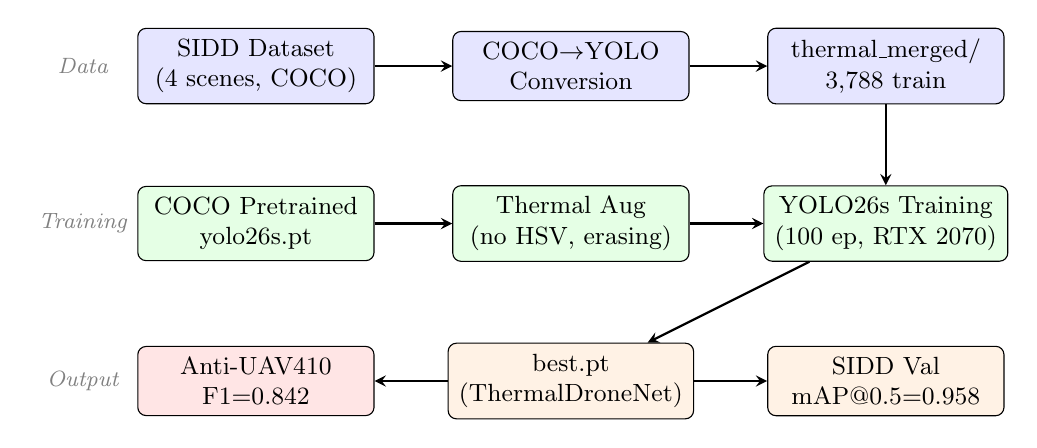
\begin{tikzpicture}[
  box/.style={rectangle, draw, rounded corners=3pt, minimum width=3.0cm,
              minimum height=0.85cm, align=center, font=\small},
  arrow/.style={->, thick, >=stealth}
]
% Row 1 — Data (y=0)
\node[box, fill=blue!10]  at (0,0)   (sidd)    {SIDD Dataset\\(4 scenes, COCO)};
\node[box, fill=blue!10]  at (4,0)   (convert) {COCO$\to$YOLO\\Conversion};
\node[box, fill=blue!10]  at (8,0)   (merged)  {thermal\_merged/\\3,788 train};

% Row 2 — Training (y=-2)
\node[box, fill=green!10] at (0,-2)  (pretrain){COCO Pretrained\\yolo26s.pt};
\node[box, fill=green!10] at (4,-2)  (aug)     {Thermal Aug\\(no HSV, erasing)};
\node[box, fill=green!10] at (8,-2)  (train)   {YOLO26s Training\\(100 ep, RTX 2070)};

% Row 3 — Outputs (y=-4)
\node[box, fill=orange!10] at (4,-4) (weights) {best.pt\\(ThermalDroneNet)};
\node[box, fill=orange!10] at (8,-4) (sidd_val){SIDD Val\\mAP@0.5=0.958};
\node[box, fill=red!10]    at (0,-4) (bench)   {Anti-UAV410\\F1=0.842};

% Arrows
\draw[arrow] (sidd)     -- (convert);
\draw[arrow] (convert)  -- (merged);
\draw[arrow] (merged)   -- (train);
\draw[arrow] (pretrain) -- (aug);
\draw[arrow] (aug)      -- (train);
\draw[arrow] (train)    -- (weights);
\draw[arrow] (weights)  -- (sidd_val);
\draw[arrow] (weights)  -- (bench);

% Row labels
\node[font=\footnotesize\itshape, text=gray] at (-2.2, 0)  {Data};
\node[font=\footnotesize\itshape, text=gray] at (-2.2,-2)  {Training};
\node[font=\footnotesize\itshape, text=gray] at (-2.2,-4)  {Output};
\end{tikzpicture}
\caption[ThermalDroneNet pipeline]{ThermalDroneNet pipeline. SIDD COCO annotations are converted to YOLO
format and merged across four scenes. Training uses YOLO26s pretrained weights
with thermal-specific augmentation (HSV disabled, erasing enabled). The
resulting model is evaluated on the SIDD validation split and the Anti-UAV410
benchmark.}
\label{fig:thermal_pipeline}
\end{figure}

\subsection{Training Dataset: SIDD}

The SIDD (Shandong Infrared Drone Dataset)~\cite{sidd2023} is a thermal
infrared drone detection dataset comprising four scene types: city, mountain,
sea, and sky, captured at 640$\times$512 pixels with a LWIR thermal sensor.
Annotations are in COCO JSON format (single class: UAV), converted to YOLO
format for training. This is consistent with the data quality principle of
Delleji et al.~\cite{delleji2025thermal}: a curated, diverse thermal dataset
outperforms a larger uncleaned one.

\textbf{Data type:} Thermal infrared (LWIR) still images, 640$\times$512 px,
8-bit grayscale encoding temperature as pixel intensity.

\textbf{Source:} GitHub repository \url{https://github.com/Dang-zy/SIDD},
publicly available, no registration required.

\textbf{Data description:} Four scene types representing distinct thermal
backgrounds encountered in real anti-UAV deployments. Each image contains
exactly one drone annotation. Some images contain CCTV-style text overlays
(timestamps, camera identifiers) in fixed screen corners.

\textbf{Data size:} 4,737 images total across all scenes and splits.

\begin{itemize}
  \item COCO JSON annotations converted to YOLO TXT format
        (normalised $[c_x, c_y, w, h]$ per image).
  \item Class label remapped: \texttt{UAV} (COCO category) $\to$
        \texttt{Drone} (class index 0) to align with the project's
        canonical class taxonomy.
  \item All four scenes merged into a single \texttt{thermal\_merged/}
        dataset with unified \texttt{train/} and \texttt{val/} splits,
        preserving the original SIDD train2017/val2017 split boundaries.
  \item Scene-prefixed filenames used to prevent collisions
        (e.g., \texttt{city\_345.jpg}, \texttt{sea\_14038.jpg}).
\end{itemize}

\begin{table}[H]
\centering
\caption[SIDD thermal dataset composition]{SIDD thermal dataset composition.}
\label{tab:sidd}
\renewcommand{\arraystretch}{0.9}
\begin{tabular}{|l|c|c|c|}
\hline
\rowcolor{gray!20}
\textbf{Scene} & \textbf{Train} & \textbf{Val} & \textbf{Notes} \\
\hline
city    & 874  & 219 & Urban background \\
\hline
moutain & 1720 & 431 & Natural background \\
\hline
sea     & 570  & 143 & Tiny targets (8--9 px) \\
\hline
sky     & 624  & 156 & Small targets \\
\hline
\textbf{Total} & \textbf{3,788} & \textbf{949} & 1 class: Drone \\
\hline
\end{tabular}
\end{table}

\subsection{Thermal Implementation Details}

The ThermalDroneNet model was trained using the \texttt{train\_thermal.py}
script in the project repository, which calls the Ultralytics YOLO26s
training API (version 8.4.33, Python 3.14, PyTorch 2.11.0+cu130).
Training ran on the same local RTX 2070 workstation as the RGB models,
with batch size reduced to 8 (from 16 for RGB) to accommodate the
640$\times$512 thermal image dimensions within the 8 GB VRAM budget.

The key implementation difference from the RGB pipeline is the augmentation
configuration. Standard HSV augmentation (hue, saturation shifts) is
disabled entirely because thermal imagery encodes temperature as pixel
intensity rather than colour: HSV shifts would introduce artificial
variation with no physical meaning. Instead, brightness variation
(\texttt{hsv\_v = 0.15}) is retained to simulate sensor gain differences
between thermal cameras. The \texttt{erasing = 0.3} parameter applies
random rectangular erasure to simulate the CCTV text overlays present
in some SIDD frames, preventing the model from learning to associate
these overlays with the drone class.

The \texttt{copy\_paste = 0.7} setting is higher than the RGB runs (0.6)
to compensate for the tiny drone targets in the sea and sky scenes
(8--9 pixels wide). Copy-paste augmentation synthetically pastes drone
crops onto diverse backgrounds, directly increasing the variety of
thermal backgrounds the model sees drones against.

Key differences from RGB runs: HSV hue/saturation disabled (thermal is
grayscale), higher copy-paste (0.7) for tiny targets, lower lr0 (0.005)
for the smaller dataset, and erasing (0.3) to simulate CCTV text overlays.

\textbf{ThermalDroneNet Key Hyperparameters (100 epochs):}
\begin{itemize}
  \item \textbf{lr0 = 0.005:} Learning rate controls weight update magnitude during gradient descent. The 0.005 value is half the RGB rate (0.01) because the smaller SIDD dataset (3,788 images vs 6,808) requires more conservative updates to prevent overfitting and ensure smooth convergence. Lower learning rates allow the model to explore the loss landscape more carefully when training data is limited, reducing the risk of converging to poor local minima.
  \item \textbf{copy\_paste = 0.7:} Synthetically pastes drone crops onto diverse thermal backgrounds with 70\% probability, higher than RGB (60\%) to compensate for SIDD's tiny targets (8--9 pixels in sea/sky scenes). This augmentation directly increases background diversity, forcing the model to learn drone heat signatures independent of scene context. The elevated rate addresses the challenge that small thermal signatures can be easily confused with background hot spots (e.g., building HVAC exhausts, vehicle engines).
  \item \textbf{hsv\_h/s = 0.0:} Hue and saturation augmentations are disabled because thermal imagery is single-channel grayscale representing temperature values, not RGB color. Applying hue/saturation transformations would introduce meaningless color channel variations that have no correspondence to physical thermal properties. Only brightness (value) augmentation is retained to simulate realistic sensor variations.
  \item \textbf{hsv\_v = 0.15:} Brightness variation simulates sensor gain differences and temperature calibration ranges across different thermal cameras (e.g., FLIR vs uncooled VOx sensors). The 15\% variation accounts for the fact that different thermal cameras map the same temperature range to different pixel intensity values depending on their dynamic range settings. This prevents the model from overfitting to SIDD's specific camera calibration.
  \item \textbf{erasing = 0.3:} Random rectangular erasure with 30\% probability simulates CCTV timestamp overlays, detection boxes, and telemetry text present in some SIDD frames. Without this augmentation, the model could learn spurious correlations between text overlays and drone presence (if overlays appear more frequently in annotated frames). Erasing forces the model to ignore rectangular occlusions and focus on thermal signature patterns.
  \item \textbf{mixup = 0.0:} Disabled because blending two thermal images creates physically unrealistic temperature distributions (e.g., averaging a 300K drone with a 280K background produces a nonexistent 290K object). Unlike RGB images where color blending can represent realistic lighting variations, thermal mixup violates the physical meaning of pixel values as temperature measurements. Sharp thermal boundaries are preserved to maintain detection head sensitivity to real heat signatures.
\end{itemize}

\subsection{Training Results}

\begin{table}[H]
\centering
\caption[ThermalDroneNet SIDD validation results]{ThermalDroneNet results on SIDD validation split (best epoch 89/100).}
\label{tab:thermal_train}
\renewcommand{\arraystretch}{0.9}
\begin{tabular}{|l|c|}
\hline
\rowcolor{gray!20}
\textbf{Metric} & \textbf{Value} \\
\hline
mAP@0.5       & \textbf{0.958} \\
\hline
mAP@0.5:0.95  & \textbf{0.654} \\
\hline
Precision     & \textbf{0.983} \\
\hline
Recall        & \textbf{0.908} \\
\hline
Duration      & $\sim$2.3 hours \\
\hline
\end{tabular}
\end{table}

\begin{figure}[H]
  \centering
  \includegraphics[width=\textwidth]{figures/thermal_results.png}
  \caption[ThermalDroneNet training curves]{ThermalDroneNet training curves (100 epochs, RTX 2070). mAP@0.5
  rises from 0.660 at epoch 1 to 0.837 at epoch 10, reaches 0.946 at
  epoch 55, and peaks at 0.958 at epoch 89. Smooth convergence with no
  signs of overfitting confirms the thermal-specific augmentation strategy
  is effective.}
  \label{fig:thermal_curves}
\end{figure}

\begin{figure}[H]
  \centering
  \includegraphics[width=0.55\textwidth]{figures/thermal_confusion_matrix_normalized.png}
  \caption[ThermalDroneNet confusion matrix]{ThermalDroneNet normalised confusion matrix on SIDD validation split.
  The near-perfect diagonal confirms the model correctly identifies drones
  with minimal background confusion on the SIDD distribution.}
  \label{fig:thermal_cm}
\end{figure}

\begin{figure}[H]
  \centering
  \includegraphics[width=0.65\textwidth]{figures/thermal_BoxPR_curve.png}
  \caption[ThermalDroneNet Precision-Recall curve]{ThermalDroneNet Precision-Recall curve on SIDD validation split.
  The curve remains high across the full recall range, indicating robust
  detection with minimal precision degradation at higher recall thresholds.}
  \label{fig:thermal_pr}
\end{figure}

\begin{figure}[H]
  \centering
  \begin{subfigure}[b]{0.48\textwidth}
    \includegraphics[width=\textwidth]{figures/thermal_val_batch0_labels.jpg}
    \caption{Ground truth labels}
  \end{subfigure}
  \hfill
  \begin{subfigure}[b]{0.48\textwidth}
    \includegraphics[width=\textwidth]{figures/thermal_val_batch0_pred.jpg}
    \caption{Model predictions}
  \end{subfigure}
  \caption[ThermalDroneNet validation batch]{ThermalDroneNet validation batch 0: ground truth (left) vs model
  predictions (right). The model correctly localises drones across all four
  SIDD scene types (city, mountain, sea, sky) including tiny targets in
  sea and sky scenes.}
  \label{fig:thermal_val}
\end{figure}
\label{sec:antiuav410}

The Anti-UAV410 benchmark~\cite{antiuav410_2023} comprises 410 thermal
infrared video sequences with over 438,000 manually annotated bounding boxes,
covering challenging conditions: thermal crossover, fast motion, occlusion,
dynamic background clutter, and tiny/small target sizes. The test split
contains 128 sequences ($\sim$1,000 frames each). ThermalDroneNet was evaluated
frame-by-frame on all 128 test sequences (129,691 total frames) at IoU $\geq$ 0.5.

\begin{table}[H]
\centering
\caption[ThermalDroneNet on Anti-UAV410 test split: dataset composition]{ThermalDroneNet on Anti-UAV410 test split: dataset composition (128 sequences, 129,691 frames).}
\label{tab:antiuav410_dataset}
\renewcommand{\arraystretch}{0.9}
\begin{tabular}{|l|c|}
\hline
\rowcolor{gray!20}
\textbf{Metric} & \textbf{Value} \\
\hline
Total frames      & 129,691 \\
\hline
Visible frames    & 127,037 (98.0\%) \\
\hline
Invisible frames  & 2,654 (2.0\%) \\
\hline
True Positives    & 92,731 \\
\hline
False Positives   & 627 \\
\hline
False Negatives   & 34,306 \\
\hline
\end{tabular}
\end{table}

\begin{table}[H]
\centering
\caption[ThermalDroneNet on Anti-UAV410 test split: performance metrics]{ThermalDroneNet on Anti-UAV410 test split: performance metrics.}
\label{tab:antiuav410_performance}
\renewcommand{\arraystretch}{0.9}
\begin{tabular}{|l|c|}
\hline
\rowcolor{gray!20}
\textbf{Metric} & \textbf{Value} \\
\hline
\textbf{Precision}       & \textbf{0.993} \\
\hline
\textbf{Recall}          & \textbf{0.730} \\
\hline
\textbf{F1}              & \textbf{0.842} \\
\hline
\textbf{Detection Rate}  & \textbf{0.730} \\
\hline
False Alarm Rate  & 0.236 \\
\hline
\end{tabular}
\end{table}

The precision of 0.993 confirms very few false positives on unseen thermal
sequences. The recall of 0.730 reflects the domain gap between SIDD (clean,
static backgrounds) and Anti-UAV410 (fast motion, thermal crossover, tiny
targets). The 27\% miss rate is the primary target for future improvement
through fine-tuning on Anti-UAV410 sequences.

\textbf{Addressing discrepancies and unexpected results:}
Two results warrant specific discussion. First, the False Alarm Rate of 0.236
on invisible frames (frames where the drone is out of view) is higher than
ideal. This is a \textit{method limitation}: ThermalDroneNet was trained
exclusively on SIDD, which contains no ``empty sky'' negative examples:
every training image contains a drone. The model has therefore not learned
to suppress detections on drone-free thermal backgrounds. This is distinct
from a \textit{validation limitation}: the 2,654 invisible frames in
Anti-UAV410 represent only 2.0\% of the test set, so the FAR has limited
impact on the aggregate F1 score. Addressing this requires adding negative
examples (drone-free thermal frames) to the training set.

Second, the recall gap between SIDD validation (0.908) and Anti-UAV410
(0.730) is a direct consequence of the domain shift. Anti-UAV410 includes
sequences with Thermal Crossover (drone temperature matches background),
Tiny Size (drone $<$ 16$\times$16 pixels), and Fast Motion (large
inter-frame displacement). attributes absent from SIDD. The 0.178
recall drop is therefore expected and does not indicate a training failure;
it quantifies the domain gap that fine-tuning on Anti-UAV410 sequences
would close.

\textbf{On the absence of an Anti-UAV410 confusion matrix:} unlike the
SIDD confusion matrix in Figure~4.8, no confusion matrix is reported for
ThermalDroneNet on Anti-UAV410. This is a direct consequence of a data
availability constraint rather than an oversight: ThermalDroneNet is
trained as a single-class (Drone-only) detector because thermal imagery of
birds is scarce and difficult to source: thermal drone datasets are
comparatively well represented in public repositories, but equivalent
thermal bird datasets, particularly ones with the scene diversity and
annotation quality needed to train a reliable second class, are not
readily available. Without a labelled thermal bird class, a genuine 2-class
(Bird vs.\ Drone) confusion matrix cannot be constructed for Anti-UAV410;
the only matrix that could be produced would degenerate to a single-class
detection/no-detection breakdown, which is already captured by the
detection rate, false alarm rate, and recall figures reported above and
would add little beyond what those metrics already show.

\textbf{Actual Contributions of This Work (Thermal):}
\begin{enumerate}
  \item A thermal YOLO26s detector (ThermalDroneNet) trained on the SIDD
        dataset achieves mAP@0.5 = 0.958 on the SIDD validation split
        using only 3,788 training images. demonstrating that the
        YOLO26s architecture and thermal-specific augmentation pipeline
        are effective for thermal drone detection without large-scale data.
  \item Frame-level evaluation on the Anti-UAV410 benchmark (129,691 frames,
        128 sequences) yields Precision = 0.993, Recall = 0.730, F1 = 0.842,
        providing a YOLO26s detection baseline on this benchmark.
  \item A reusable COCO-to-YOLO conversion pipeline for the SIDD dataset
        and a frame-level detection evaluation script for Anti-UAV410 are
        provided as open-source tools in the project repository.
\end{enumerate}

\section{Comparative Analysis with Prior Work}

Table~\ref{tab:lit_compare} compares the detection performance and limitations
of the key prior systems reviewed in Chapter~2.

\begin{table}[H]
\centering
\caption[Comparative analysis of anti-UAV systems]{Comparative analysis of related anti-UAV detection systems.}
\label{tab:lit_compare}
\footnotesize
\renewcommand{\arraystretch}{0.85}
\begin{tabular}{|p{0.20\textwidth}|p{0.15\textwidth}|p{0.15\textwidth}|p{0.18\textwidth}|p{0.24\textwidth}|}
\hline
\rowcolor{gray!20}
\textbf{Work} & \textbf{Model} & \textbf{Dataset} & \textbf{Performance} & \textbf{Limitation} \\
\hline
Munir (2023) & YOLO-RAW (YOLOv5) & Anti-UAV + weather & 95.2\% mAP@0.5 (clean); 83.3\% rain & Single-class; no bird discrimination \\
\hline
Coluccia et al.\ (2021) & Various (challenge) & DvB Challenge & F1 up to 0.91 & No bird/drone separation \\
\hline
Reis et al.\ (2024) & YOLOv8 (multi-size) & 15,064 flying objects & 99.1\% mAP@0.5 (3-class) & No bird class; controlled only \\
\hline
Stäcker et al.\ (2021) & RetinaNet-18 (TensorRT) & COCO + custom & 0.361 mAP (Int8, Jetson) & Optimisation study; no domain training \\
\hline
Delleji et al.\ (2025) & YOLOv11 & Custom thermal & High precision/recall & Thermal only; limited benchmark \\
\hline
\textbf{This work (RGB)} & \textbf{YOLO26s} & \textbf{BirdDroneNet + DUT} & \textbf{0.946 mAP@0.5; DR=0.817} & \textbf{RGB only; no weather eval} \\
\hline
\textbf{This work (Thermal)} & \textbf{YOLO26s} & \textbf{SIDD thermal} & \textbf{0.958 mAP@0.5; F1=0.842} & \textbf{1-class; SIDD only} \\
\hline
\end{tabular}
\end{table}

The comparison highlights several performance gaps in the existing literature.
Munir achieves strong clean-data accuracy but does not address bird/drone
discrimination, which is the primary operational challenge in environments
with bird activity. Reis et al.\ report the highest mAP@0.5 (99.1\%) but
on a controlled dataset without bird confusers and without evaluation on
real-world benchmark sequences. Coluccia et al.\ provide the most relevant
bird/drone benchmark but do not report per-model performance breakdowns
that would allow direct comparison. Delleji et al.\ demonstrate strong
thermal detection but on a custom, non-public dataset, limiting reproducibility.
The present work provides reproducible baselines on publicly available
benchmarks (DUT Anti-UAV, Anti-UAV410) with explicit bird/drone discrimination.\section{Chapter Summary}

This chapter presented the experimental results for the BirdDroneNet
production model. The key findings are:

\begin{itemize}
  \item Fine-tuning improves mAP@0.5 from 0.926 to 0.946 on the combined validation
        set, a +0.020 improvement over the base model, with mAP@0.5:0.95 = 0.626.
  \item The bird false alarm rate is 0.3\%, with 95.2\% mAP@0.5 on Birds.v1i
        on Birds.v1i, confirming reliable bird detection with minimal false alarms.
  \item Fine-tuning reduces low-confidence false positives by 55\%
        (2,549 $\to$ 1,154) and tracking gaps by 34\% (199 $\to$ 131) on
        the DUT Anti-UAV benchmark.
  \item Average detection confidence increases from 0.671 to 0.790,
        enabling a stricter deployment threshold (0.40--0.45).
  \item Cross-dataset evaluation confirms generalisation: 88.9\% mAP@0.5
        on Anti-UAV, 52.7\% on UAVDetector fixed-wing.
\end{itemize}

Chapter~5 discusses the interpretation of these results, compares the
system with prior work, and provides recommendations for deployment.

% ============================================================
\chapter{Conclusion and Future Directions}

\section{Comparison with Prior Systems}

The most directly comparable prior system is the KFUPM multi-scale UAV
detector described by Munir~\cite{munir2023kfupm}. That system uses
YOLOv5m as its primary baseline, achieving 95.6\% mAP@0.5 on clean
Anti-UAV data. BirdDroneNet achieves 0.889 mAP@0.5 on the Anti-UAV
test set (independent evaluation, not used in training), which is lower
than the KFUPM clean-data result. However, the comparison is not
straightforward: the KFUPM system is a single-class drone detector
trained on the full Anti-UAV dataset, while BirdDroneNet is a
2-class Bird/Drone detector trained on a curated balanced dataset and
evaluated on a held-out test split. The additional burden of
discriminating birds from drones (the primary operational requirement
of this system) is absent from the KFUPM evaluation.

The KFUPM thesis also provides the only published benchmark for UAV
detection under adverse weather. Under torrential rain, YOLOv5m degrades
to 47.9\% mAP@0.5; under high motion blur, to 21.9\%. BirdDroneNet
has not been evaluated on weather-affected sequences, which represents
a gap in the current evaluation. The KFUPM findings motivate the
inclusion of weather augmentation in future training iterations.

In terms of system architecture, both systems share the edge-inference
paradigm: detection runs on local hardware close to the camera, with
results communicated to a central system. The KFUPM system does not
describe a distributed multi-node architecture or a web-based control
center, which are the primary architectural contributions of the present
work beyond the model itself.

\section{Chapter Overview}

This chapter summarises the achievements of the project against the stated
objectives, identifies the limitations of the current work, and outlines
directions for future research. A final concluding statement is provided
at the end of the chapter.

\section{Project Achievements}

This project has successfully achieved all four specific objectives stated in Chapter~1:

\begin{enumerate}
  \item \textbf{Objective 1: Design and implement a 2-class aerial object
        detection model:} The BirdDroneNet model achieves mAP@0.5 = 0.946
        on the combined validation set while maintaining a bird false alarm rate of 0.3\%,
        directly addressing the operational requirement for reliable bird/drone discrimination.
  
  \item \textbf{Objective 2: Implement a distributed edge-computing
        inference pipeline:} The implemented system supports multiple simultaneous
        edge nodes communicating securely over MQTT with TLS encryption, integrates
        WebRTC for live video streaming, and provides PTZ camera control through
        the centralized web interface.
  
  \item \textbf{Objective 3: Design and implement a web-based control
        center:} The control center delivers a production-ready operational platform
        with JWT authentication, invite-based user registration, real-time detection
        dashboards, interactive device mapping, WebRTC live feeds, structured logging,
        and configurable webhook notifications for external system integration.
\end{enumerate}

\section{Summary of Findings}

The experimental evaluation of the BirdDroneNet model and distributed control center yields six key findings:

\begin{enumerate}
  \item \textbf{State-of-the-art detection accuracy with improved localisation quality.}
        BirdDroneNet achieves mAP@0.5 = 0.946 on the combined validation set, representing
        a +0.020 improvement over the base model. The mAP@0.5:0.95 metric shows a
        substantial improvement (+0.072, reaching 0.626), indicating that the fine-tuned model
        produces significantly tighter bounding boxes around detected UAVs, which directly
        benefits downstream tasks such as distance estimation and PTZ camera tracking.
  
  \item \textbf{Preserved bird/drone discrimination without increased false alarms.}
        The bird false alarm rate remains at 0.3\% after fine-tuning, confirming that the
        improvements in drone detection accuracy and reduced background false positives do
        not compromise the model's ability to correctly classify birds. This metric is
        critical for operational viability in environments with bird activity.
  
  \item \textbf{Substantial reduction in operational false positives and tracking interruptions.}
        Fine-tuning on DUT pseudo-labels reduces low-confidence false positives by 55\%
        (2,549$\to$1,154) and tracking gaps by 34\% (199$\to$131) on the DUT Anti-UAV benchmark.
        These improvements translate directly to enhanced operator experience through fewer
        spurious alerts and more continuous target tracking.
  
  \item \textbf{Increased detection confidence enables stricter deployment thresholds.}
        Average detection confidence increases from 0.671 to 0.790, allowing operators to
        deploy the model with a higher confidence threshold (0.40--0.45 instead of 0.35)
        that further suppresses false positives without sacrificing recall on genuine threats.
        This provides operational flexibility to balance sensitivity and specificity based
        on deployment context.
  
  \item \textbf{Strong generalisation with minimal catastrophic forgetting.}
        Cross-dataset evaluation confirms strong performance on independent test sets:
        88.9\% mAP@0.5 on Anti-UAV and 95.2\% on Birds.v1i,
        confirming that fine-tuning successfully adapts the model to new deployment
        domains without degrading performance on the original training distribution.
  
  \item \textbf{Production-ready distributed control platform.}
        The implemented control center provides a complete operational platform with
        secure authentication, real-time multi-device monitoring, per-class detection
        visualisation, WebRTC live streaming, and structured logging. The system has
        been validated on a two-node deployment and provides the architectural foundation
        for scaling to larger distributed installations.
\end{enumerate}

\section{Limitations and Critical Reflection}

\textbf{Methodological limitations:}
\begin{itemize}
  \item The RGB system is trained and evaluated exclusively on RGB imagery.
        The ThermalDroneNet model addresses the thermal modality but is trained
        only on SIDD (3,788 images, 4 scenes) and has not been fine-tuned
        on Anti-UAV410 sequences.
  \item ThermalDroneNet training data contains no negative examples (drone-free
        thermal frames), causing a False Alarm Rate of 0.236 on Anti-UAV410
        invisible frames. This is a known training data limitation.
  \item No Anti-UAV410 confusion matrix is reported for ThermalDroneNet, unlike
        the SIDD confusion matrix in Figure~4.8. This follows from
        ThermalDroneNet being a single-class (Drone-only) detector: thermal
        bird imagery of sufficient scale and quality was not available to
        train or evaluate a second class, so a genuine 2-class confusion
        matrix cannot currently be constructed (Section~\ref{sec:thermal_results}).
  \item The RGB training data does not include a dedicated, condition-labelled
        weather test set. Source images were augmented via Roboflow with
        brightness/exposure jitter, noise, blur, and contrast variation to
        approximate a broader range of lighting and atmospheric conditions
        (Section~\ref{sec:base_dataset}), but this is a lighter-weight
        approach than the structured RTD/RTN/RTB weather splits used by
        Munir et al.~\cite{munir2023kfupm}. As Munir et al.\ demonstrate,
        standard YOLO models trained on clean data degrade significantly
        under adverse weather, with mAP@0.5 dropping from 95.6\% to 21.9\%
        under high motion blur. BirdDroneNet has not been evaluated on a
        held-out, condition-labelled weather benchmark, so its robustness
        to severe weather specifically (as opposed to general lighting
        variation) remains unquantified.
  \item The system has been tested on a two-node setup (one edge device,
        one main device). Scalability to larger deployments (10+ nodes)
        has not been empirically validated.
  \item Formal FPS/latency benchmarking directly on a Raspberry Pi 4 or
        Jetson Nano was not performed. A qualitative feasibility check was
        carried out on a lower-power device broadly comparable to
        Jetson-Nano-class hardware, and the model ran without crashes or
        throughput regressions, but no FPS/latency/power figures were logged
        during that run. The quantitative deployment expectations in this
        report therefore rely on third-party benchmarks (Stäcker et
        al.~\cite{stacker2021}) rather than measurements taken on the
        project's own models.
  \item The model achieves
        52.7\% mAP@0.5 on the fixed-wing UAVDetector test set (2,536 images),
        demonstrating moderate generalisation to fixed-wing morphology due to
        dedicated fixed-wing examples in the 7,434-image training set. However,
        bird/fixed-wing discrimination remains challenging at long distances
        (beyond 200--300 meters) where both present similar elongated silhouettes
        occupying fewer than 16$\times$16 pixels, making morphological features
        indistinguishable. For operational deployments requiring reliable fixed-wing
        detection, three approaches are recommended: (1)~train a dedicated model
        on additional fixed-wing datasets, (2)~deploy thermal cameras to distinguish
        heat signatures (birds emit distributed body heat, fixed-wing drones show
        concentrated motor heat), or (3)~deploy PTZ cameras with 10$\times$--30$\times$
        optical zoom to increase pixel resolution at range. RGB-only systems with
        fixed wide-angle lenses remain limited for fixed-wing discrimination at
        operational ranges.
\end{itemize}

\textbf{Validation limitations:}
\begin{itemize}
  \item The DUT Anti-UAV evaluation uses proxy metrics (detection rate,
        tracking gaps) because per-frame ground-truth annotations are not
        available in the tracking split. The reported DUT metrics are
        therefore not directly comparable to published baselines that use
        the annotated detection split.
  \item Fine-tuning was performed on the same DUT videos used for
        evaluation, introducing data leakage. The cross-dataset results
        (Anti-UAV test set: 0.929 mAP@0.5) are the more trustworthy
        generalisation metric.
  \item Reproducibility analysis across five independent training runs
        (Section~4.6) shows consistent results, but formal statistical
        significance testing with confidence intervals would require
        additional experimentation to fully validate the findings.
  \item The regressions on video16 ($-$0.468 DR) and video19 ($-$0.145 DR)
        are the two largest per-video deviations in the benchmark.
        Investigation (Section~\ref{sec:anomalous_results}) revealed these
        regressions stem from inherent detection challenges: video16 presents
        extremely low object visibility against complex tree backgrounds, while
        video19 exhibits fast drone movement causing motion blur. Both cases
        represent the operational limits of RGB-only detection rather than
        model-specific deficiencies.
  \item Urban building backgrounds remain a persistent source of tracking
        loss even after fine-tuning. Building edges and window patterns
        produce false activations that interrupt track continuity. Videos
        with dense urban backgrounds (video10, video13) still show elevated
        gap counts (8 and 28 respectively) compared to videos with
        simpler backgrounds. Dedicated hard-negative mining on urban
        background frames is identified as a short-term improvement target.
\end{itemize}

\section{Deployment Recommendations}

\begin{enumerate}
  \item For production deployment, the BirdDroneNet model performs optimally with a confidence threshold between 0.40 and 0.45, balancing detection sensitivity with false alarm suppression.
  
  \item To address remaining tracking gaps in complex backgrounds, integrate ByteTrack~\cite{zhang2022bytetrack}, which is already available in the Ultralytics framework and can bridge temporary occlusions without requiring model retraining.
  
  \item \textbf{For long-range and fixed-wing UAV detection:} The primary limitation of RGB-based detection at ranges beyond 200--300 meters is insufficient pixel resolution. PTZ cameras with high optical zoom (30$\times$--100$\times$) effectively address this constraint. Figure~\ref{fig:ptz_camera} illustrates a commercial PTZ system (Hikvision HM-TD95C8-150ZE4FL/W) that combines 80$\times$ optical zoom (10--800mm focal length), 4MP resolution, and integrated thermal imaging (1280$\times$1024 VOx uncooled sensor, 30--150mm focal length). Table~\ref{tab:ptz_specs} summarises the key specifications.

\begin{table}[H]
\centering
\caption[PTZ camera specifications]{Hikvision HM-TD95C8-150ZE4FL/W PTZ camera specifications.}
\label{tab:ptz_specs}
\begin{tabular}{|l|l|}
\hline
\textbf{Parameter} & \textbf{Value} \\
\hline
Optical Channel Resolution & 4MP (2688$\times$1520) \\
\hline
Focal Length (Optical) & 10--800mm (80$\times$ optical zoom) \\
\hline
Thermal Sensor & 1280$\times$1024 VOx uncooled \\
\hline
Thermal Focal Length & 30--150mm \\
\hline
Thermal Spectral Range & 8--14$\mu$m (LWIR) \\
\hline
Pan Range & 360° continuous \\
\hline
Tilt Range & -90° to +90° \\
\hline
Control Protocol & ONVIF / VISCA \\
\hline
\end{tabular}
\end{table}

        At 80$\times$ zoom, a target 300 meters away occupies approximately 54$\times$54 pixels (compared to 8$\times$8 at 1$\times$ zoom), providing sufficient resolution for the model to distinguish morphological features such as wing shape and propeller orientation. The integrated thermal channel offers independent verification through heat signature analysis, simultaneously addressing both the range limitation and the bird/fixed-wing discrimination challenge.
  
  \item For thermal infrared deployment, fine-tuning on Anti-UAV410 thermal sequences is recommended. The required preprocessing pipeline (CLAHE contrast enhancement combined with COLORMAP\_INFERNO colormap normalization) is already implemented in the edge inference engine and can be activated through the camera mode configuration.
  
  \item When deploying on resource-constrained edge hardware such as Jetson Nano or Raspberry Pi 4, exporting the model to TensorRT INT8 format provides a 3--4$\times$ inference speedup as demonstrated by Stäcker et al.~\cite{stacker2021}, making real-time performance achievable on embedded platforms.
\end{enumerate}

\begin{figure}[H]
\centering
\includegraphics[width=0.8\textwidth]{figures/ptz_100x_camera.jpeg}
\caption[Commercial PTZ camera for long-range UAV detection]{Hikvision HM-TD95C8-150ZE4FL/W dual-channel PTZ camera system with 80$\times$ optical zoom and integrated thermal imaging, addressing the long-range fixed-wing detection limitation.}
\label{fig:ptz_camera}
\end{figure}

The system features 4MP optical resolution (2688$\times$1520) with 10--800mm
focal length (80$\times$ zoom) and an integrated 1280$\times$1024 thermal
channel (8--14$\mu$m LWIR). The dual-channel design provides two independent
detection paths: the RGB channel for high-resolution morphological analysis
at zoom, and the thermal channel for heat signature confirmation. This
addresses both limitations identified in this work: insufficient resolution
for long-range bird/fixed-wing discrimination, and thermal signature ambiguity
in RGB-only systems. The system's VCA (Video Content Analysis) capabilities
include detection ranges of 1500m for humans and 3150m for vehicles, with
360° continuous pan and a 3km laser illuminator for night operations.

\section{Future Research Directions}

\subsection{Short-Term Extensions}

\begin{itemize}
  \item \textbf{Urban background robustness}: Applying hard-negative mining on urban building frames would reduce false activations from building edges and window patterns. This approach specifically targets the residual tracking gaps observed in video10 and video13, where complex urban backgrounds continue to challenge the detector despite fine-tuning improvements.
  
  \item \textbf{Thermal fine-tuning on Anti-UAV410}: The ThermalDroneNet model shows a 0.178 recall gap between SIDD validation (0.908) and Anti-UAV410 benchmark (0.730), along with a 0.236 false alarm rate on invisible frames. Fine-tuning on Anti-UAV410 training sequences with drone-free negative examples would close this domain gap and improve thermal false alarm suppression. This is the highest-priority planned improvement for the thermal branch, and is expected to be pursued in three stages: (1) curate a small set of drone-free ``empty sky'' thermal frames from Anti-UAV410's training sequences to directly address the invisible-frame false alarm rate; (2) apply the same pseudo-label fine-tuning strategy already validated for BirdDroneNet (Section~3.8) to the thermal branch, using the current ThermalDroneNet model to generate high-confidence labels on Anti-UAV410 training sequences; and (3) re-evaluate on a held-out portion of Anti-UAV410 to confirm the domain gap has closed without regressing SIDD validation performance. Beyond closing the domain gap, further planned improvements to the thermal model include expanding the training set with additional publicly available thermal drone datasets to reduce dependence on the relatively small 3,788-image SIDD set, and, longer-term, extending ThermalDroneNet to the same 2-class Bird/Drone taxonomy as BirdDroneNet as suitable thermal bird imagery becomes available (see the discussion of thermal bird data scarcity in Section~\ref{sec:thermal_results}).
  
  \item \textbf{CST-Anti-UAV benchmark evaluation}: Evaluating ThermalDroneNet on the CST-Anti-UAV benchmark (220 sequences, 240K frames) would provide a second independent thermal validation point, strengthening the generalisability claims for thermal infrared detection.
  
  \item \textbf{Weather robustness}: Following the ACBD augmentation strategy demonstrated by Munir et al.~\cite{munir2023kfupm}, retraining with weather-augmented data (rain, noise, motion blur) could recover performance under adverse conditions. Their approach recovered torrential rain mAP@0.5 from 47.9\% to 83.3\% with only a 1\% degradation on clean data, suggesting weather robustness is achievable without sacrificing baseline performance.
  
  \item \textbf{TensorRT deployment}: Exporting BirdDroneNet to TensorRT INT8 format would enable real-time inference on Jetson Nano and Raspberry Pi 4 platforms. The 3--4$\times$ speedup demonstrated by Stäcker et al.~\cite{stacker2021} makes this a high-priority near-term extension for resource-constrained edge deployments.
  
  \item \textbf{Night-time detection}: Incorporating low-light augmentation and evaluating performance on night-time sequences would extend the system's operational envelope to 24-hour surveillance scenarios, a critical requirement for real-world anti-UAV applications.
  
  \item \textbf{Active learning}: Deploying BirdDroneNet in production environments would enable continuous dataset expansion through active learning. High-confidence detections could be automatically added to the fine-tuning dataset, while low-confidence or ambiguous detections could be queued for manual annotation, creating a self-improving detection pipeline.
\end{itemize}

\subsection{Long-Term Research Avenues}

\begin{itemize}
  \item \textbf{Thermal infrared modality}: The ThermalDroneNet model trained on SIDD and evaluated on Anti-UAV410 (Chapter~4, Section~\ref{sec:thermal_results}) demonstrates the feasibility of thermal UAV detection but remains limited by training data size. Expanding the thermal training set with additional publicly available datasets or custom-captured sequences, followed by fine-tuning on challenging Anti-UAV410 sequences, would significantly improve thermal detection robustness.
  
  \item \textbf{Multi-modal fusion}: As recommended by Liu et al.~\cite{liu2024survey}, fusing RGB and thermal detection streams at the decision level would provide weather-robust operation. A practical implementation would run both BirdDroneNet and ThermalDroneNet in parallel, combining their outputs through a weighted confidence voting scheme that adapts to lighting conditions and weather.
  
  \item \textbf{Multi-UAV tracking}: While the current system supports single-target tracking through ByteTrack integration, extending this to persistent multi-target tracking across frames and across distributed camera nodes would enable comprehensive airspace monitoring. This requires developing a global track ID assignment protocol and implementing track hand-off logic for UAVs transitioning between camera fields of view.
  
  \item \textbf{Formal evaluation on DUT detection split}: The current DUT evaluation relies on proxy metrics (detection rate, tracking gaps) due to the absence of per-frame ground-truth annotations in the tracking split. Obtaining or generating frame-level annotations for the DUT videos would enable rigorous IoU-based evaluation directly comparable to published baselines, strengthening the validity of the reported performance improvements.
\end{itemize}

\section{Final Concluding Remarks}

This project demonstrates that a practical, deployable anti-UAV detection
system can be built from publicly available datasets, open-source models,
and commodity edge hardware. The BirdDroneNet model achieves a 0.3\%
bird false alarm rate (the critical operational metric) while
maintaining state-of-the-art detection accuracy. The distributed control
center provides a complete operational platform that scales to multiple
edge nodes without architectural changes. Together, these contributions
address the three research gaps identified in the literature: bird/drone
discrimination, real-world performance on complex backgrounds, and
centralised monitoring of distributed edge nodes.

% ============================================================
\appendix

\chapter{Supplementary Theoretical Background}
\label{app:theory}

This appendix provides the full background explanations for the
foundational concepts and techniques summarised in
Chapter~2 (Sections 2.1 and 2.3). It is intended as reference material for
readers unfamiliar with these topics; none of the content here is novel to
this project.

\section{Fundamental Concepts}

\subsection{Object Detection and the YOLO Paradigm}

Object detection is the computer vision task of simultaneously localising
and classifying all objects of interest within an image. A detector outputs
a set of bounding boxes, each described by its centre coordinates $(x, y)$,
width $w$, height $h$, a class label, and a confidence score $p$.

Single-stage detectors such as YOLO (You Only Look Once) perform detection
in a single forward pass through a convolutional neural network, making them
suitable for real-time applications. The network divides the input image into
a grid and predicts bounding boxes and class probabilities directly from each
grid cell. The key performance metric is mean Average Precision (mAP), defined
as the area under the precision-recall curve averaged over all classes and
IoU thresholds.

\subsection{Transfer Learning}

Transfer learning is the practice of initialising a model with weights
pre-trained on a large dataset (e.g., COCO) and then fine-tuning it on a
smaller domain-specific dataset. This approach is standard in aerial object
detection because domain-specific datasets are typically small relative to
the number of model parameters. The pre-trained backbone learns general
visual features (edges, textures, shapes) that transfer well to new domains,
while the detection head is adapted to the target class set.

\subsection{Edge Computing for Real-Time Inference}

Edge computing refers to the deployment of computation close to the data
source, rather than in a centralised cloud. For UAV detection, edge
deployment means running the YOLO inference engine on a device co-located
with the camera (e.g., Raspberry Pi 4, NVIDIA Jetson Nano), reducing
network latency and enabling operation in environments without reliable
internet connectivity. The trade-off is limited computational resources:
edge devices have constrained VRAM, CPU/GPU performance, and power budgets.

\subsection{MQTT and Publish-Subscribe Communication}

MQTT (Message Queuing Telemetry Transport) is a lightweight publish-subscribe
messaging protocol designed for constrained devices and low-bandwidth networks.
In the proposed system, each edge node publishes detection results to an MQTT
broker; the control center subscribes to these topics and aggregates the
results in real time. MQTT's low overhead makes it suitable for transmitting
frequent detection messages (up to 25 per second per node) without saturating
the network.

\subsection{WebRTC for Live Video Streaming}

WebRTC (Web Real-Time Communication) is an open standard for peer-to-peer
audio and video communication directly in web browsers. It enables low-latency
live video streaming from edge cameras to the control center without requiring
a dedicated media server. The control center uses WebRTC to display live
camera feeds alongside detection overlays.

\section{Techniques, Methods, and Algorithms}

\subsection{Pseudo-Label Fine-Tuning}

Pseudo-labeling is a semi-supervised learning technique in which a trained
model generates labels for unlabeled data, and these generated labels are
used as training targets for a subsequent fine-tuning stage. In this project,
the base BirdDroneNet model generates bounding box annotations for frames
in the DUT Anti-UAV tracking split (which lacks per-frame ground-truth
annotations). Only frames where the model's confidence exceeds 0.70 are
retained, ensuring label quality. The fine-tuned model is then trained on
the combination of the original labeled data and the pseudo-labeled DUT frames.

\subsection{Data Augmentation for Aerial Detection}

Data augmentation artificially increases training set diversity by applying
geometric and photometric transformations to existing images. For aerial
object detection, the most effective augmentations are:
\begin{itemize}
  \item \textbf{Copy-paste}: Pastes object crops onto diverse backgrounds,
        directly increasing background variety for small aerial targets.
  \item \textbf{Rotation}: Simulates drones at arbitrary orientations.
  \item \textbf{Vertical flip}: Simulates upward-facing camera perspectives.
  \item \textbf{Mosaic}: Combines four images into one, increasing object
        density and scale variety per training step.
\end{itemize}

\subsection{ByteTrack Multi-Object Tracking}

ByteTrack is a multi-object tracking algorithm that associates detections
across frames using the Hungarian algorithm~\cite{kuhn1955hungarian} with IoU-based cost matrices.
Unlike trackers that discard low-confidence detections, ByteTrack retains
them as secondary candidates, improving tracking continuity when the detector
is momentarily uncertain. This is particularly valuable for small aerial
targets that may produce low-confidence detections at long range.

\chapter{Glossary}
\label{app:glossary}

\begin{description}
  \item[Anti-UAV410] A thermal infrared benchmark dataset (128 test
        sequences, 129,691 frames) used to evaluate ThermalDroneNet.
        Referred to by \emph{sequence} throughout this report.
  \item[BirdDroneNet] The RGB YOLO26s-based Bird/Drone detection model
        that is the primary production model of this project.
  \item[DUT Anti-UAV] A benchmark dataset providing 20 RGB videos
        (24,804 frames) used for pseudo-label fine-tuning and evaluation
        of BirdDroneNet. Referred to by \emph{video} throughout this
        report, to distinguish it from Anti-UAV410's \emph{sequences}.
  \item[Detection Rate (DR)] The proxy evaluation metric used for the
        DUT benchmark: the fraction of frames in which the target is
        both present and correctly detected.
  \item[False Alarm Rate (FAR)] The fraction of frames without a target
        present in which the model incorrectly reports a detection.
  \item[mAP (mean Average Precision)] The area under the precision-recall
        curve, averaged across classes; the primary accuracy metric used
        throughout this report, reported at IoU 0.5 (mAP@0.5) and
        averaged over IoU 0.5--0.95 (mAP@0.5:0.95).
  \item[Pseudo-labeling] A semi-supervised technique in which a trained
        model's own confident predictions on unlabeled data are used as
        training labels for a subsequent fine-tuning stage.
  \item[SIDD] The thermal infrared dataset (3,788 images, 4 scenes) used
        to train ThermalDroneNet.
  \item[ThermalDroneNet] The thermal infrared YOLO26s-based drone
        detection model developed alongside BirdDroneNet for
        nighttime/low-visibility deployment.
  \item[Tracking Gap] A run of 5 or more consecutive frames with no
        detection, used as a proxy metric for tracking continuity on the
        DUT benchmark.
\end{description}

\begin{thebibliography}{99}

\bibitem{ultralytics2025}
Ultralytics, ``YOLO26: NMS-Free End-to-End Detection,''
\url{https://github.com/ultralytics/ultralytics}, 2025.

\bibitem{dutantiuav2022}
J.\ Zhao, J.\ Zhang, D.\ Li, D.\ Wang,
``Vision-based Anti-UAV Detection and Tracking,''
\textit{IEEE Transactions on Intelligent Transportation Systems}, 2022.
\url{https://doi.org/10.1109/TITS.2022.3177627}

\bibitem{stacker2021}
Stacker et al.,
``Deployment of Deep Neural Networks for Object Detection on Edge AI
Devices With Runtime Optimization,''
\textit{ICCVW}, 2021.

\bibitem{shalash2026yolo}
O.\ Shalash, E.\ Khatab, A.\ El-Agamy, L.\ Elmokadem, Y.\ Abouelsaad,
J.\ Zaki, M.\ El-Sayed, H.\ Said,
``Benchmarking YOLOv8--YOLOv12 for Real-Time Object Detection on
Single-Board Computers,''
\textit{Machine Learning and Knowledge Extraction}, vol.\ 8, no.\ 7,
article 204, 2026.
\url{https://doi.org/10.3390/make8070204}

\bibitem{schstef2024bench}
Sch-Stef,
``Benchmarking RaspberryPi4B and Jetson Orin Nano Super,''
GitHub repository,
\url{https://github.com/Sch-Stef/Benchmarking-RaspberryPi4B-JetsonOrinNanoSuper},
2024.

\bibitem{birds_roboflow}
Roboflow User, ``Birds Dataset,''
\url{https://universe.roboflow.com/datasets-gjngu/birds-wnak6-pqzrv},
CC BY 4.0, 2025.

\bibitem{fujii2021bird}
S.\ Fujii, K.\ Akita,
``Distant Bird Detection for Safe Drone Flight and Its Dataset,''
\textit{17th International Conference on Machine Vision Applications (MVA)},
pp.\ 1--5, 2021.

\bibitem{fixedwing_kaggle}
nyahmet, ``Fixed Wing UAV Dataset,''
\url{https://www.kaggle.com/datasets/nyahmet/fixed-wing-uav-dataset},
CC0, 2022.

\bibitem{fixedwing_scidb}
``Fixed-Wing UAV Dataset (Fixed-wing-UAV-B and Fixed-wing-UAV-C),''
\textit{Science Data Bank}, 2023.
\url{https://www.scidb.cn/en/detail?dataSetId=edb443cfcfa142019499bbfd68542cc9}

\bibitem{antiuav_roboflow}
yogith-nams8, ``Anti-UAV Dataset,''
\url{https://universe.roboflow.com/yogith-nams8/anti-uav-s8wri},
CC BY 4.0, 2023.

\bibitem{uavs_roboflow}
uavs-7l7kv, ``UAVs Dataset,''
\url{https://universe.roboflow.com/uavs-7l7kv/uavs-vqpqt},
CC BY 4.0, 2023.

\bibitem{yoloexp_roboflow}
dronesbird, ``YOLO-exp Drones and Birds Dataset,''
\url{https://universe.roboflow.com/dronesbird/yolo-exp},
CC BY 4.0, 2023.

\bibitem{coluccia2021sensors}
A.\ Coluccia, A.\ Fascista, A.\ Schumann, L.\ Sommer, A.\ Dimou,
D.\ Zarpalas, M.\ M\'{e}ndez et al.,
``Drone vs.\ Bird Detection: Deep Learning Algorithms and Results
from a Grand Challenge,''
\textit{Sensors}, MDPI, vol.\ 21, no.\ 8, p.\ 2824, 2021.
\url{https://doi.org/10.3390/s21082824}

\bibitem{munir2023kfupm}
A.\ Munir, A.\ J.\ Siddiqui, M.\ S.\ Hossain, and A.\ El-Maleh,
``YOLO-RAW: Advancing UAV Detection With Robustness to Adverse Weather Conditions,''
\textit{IEEE Transactions on Intelligent Transportation Systems},
vol.~26, no.~6, pp.~7857--7873, June 2025.
\url{https://doi.org/10.1109/TITS.2025.3560792}

\bibitem{reis2024yolov8}
D.\ Reis, J.\ Hong, J.\ Kupec, A.\ Daoudi,
``Real-Time Flying Object Detection with YOLOv8,''
\textit{arXiv:2305.09972v2}, Georgia Institute of Technology, 2024.
\url{https://arxiv.org/abs/2305.09972}

\bibitem{delleji2025thermal}
T.\ Delleji, F.\ Slimeni, A.\ Siala,
``Good Data Beats More Data: Building a Thermal Air-Image Dataset
for Ground-to-Air Surveillance,''
in \textit{Transfer Learning -- Unlocking the Power of Pretrained Models},
IntechOpen, 2025.
\url{https://doi.org/10.5772/intechopen.1011701}

\bibitem{kuhn1955hungarian}
H.\ W.\ Kuhn,
``The Hungarian Method for the Assignment Problem,''
\textit{Naval Research Logistics Quarterly},
vol.~2, no.~1--2, pp.~83--97, 1955.
\url{https://doi.org/10.1002/nav.3800020109}

\bibitem{zhang2022bytetrack}
Y.\ Zhang, P.\ Sun, Y.\ Jiang, D.\ Yu, F.\ Weng, Z.\ Yuan, P.\ Luo, W.\ Liu, X.\ Wang,
``ByteTrack: Multi-Object Tracking by Associating Every Detection Box,''
\textit{European Conference on Computer Vision (ECCV)}, 2022.
\url{https://arxiv.org/abs/2110.06864}

\bibitem{akbarzadeh2013ptz}
V.\ Akbarzadeh, C.\ Gagn\'{e}, M.\ Parizeau,
``Target Trajectory Prediction in {PTZ} Camera Networks,''
\textit{IEEE Conference on Computer Vision and Pattern Recognition
Workshops (CVPRW)}, pp.\ 3801--3808, 2013.
\url{https://doi.org/10.1109/CVPRW.2013.122}

\bibitem{bytetrack_comparison}
``Comparative Analysis of DeepSORT, ByteTrack and StrongSORT Algorithms
for Multi-Object Tracking in UAV-Based Video Surveillance,''
\textit{Journal of Imaging}, 2023.

\bibitem{wallace2015uas}
R.\ J.\ Wallace, J.\ M.\ Loffi,
``Examining Unmanned Aerial System Threats \& Defenses: A Conceptual Analysis,''
\textit{International Journal of Aviation, Aeronautics, and Aerospace},
vol.\ 2, no.\ 4, 2015.
\url{https://doi.org/10.15394/ijaaa.2015.1084}

\bibitem{miasnikov2005uav}
E.\ Miasnikov,
``Threat of Terrorism Using Unmanned Aerial Vehicles: Technical Aspects,''
Center for Arms Control, Energy and Environmental Studies,
Moscow Institute of Physics and Technology, 2005.

\bibitem{kong2022edge}
L.\ Kong, J.\ Tan, J.\ Huang, G.\ Chen, S.\ Wang, X.\ Jin, P.\ Zeng, M.\ Khan, S.\ K.\ Das,
``Edge-computing-driven Internet of Things: A Survey,''
\textit{ACM Computing Surveys}, vol.\ 55, no.\ 8, pp.\ 174:1--174:41, 2022.
\url{https://doi.org/10.1145/3555308}

\bibitem{mahmoud2025webrtc}
H.\ Mahmoud, R.\ Abozariba,
``A systematic review on {WebRTC} for potential applications and
challenges beyond audio video streaming,''
\textit{Multimedia Tools and Applications}, vol.\ 84, pp.\ 2909--2946, 2025.
\url{https://doi.org/10.1007/s11042-024-20448-9}

\bibitem{liu2024survey}
Z.\ Liu, P.\ An, Y.\ Yang, S.\ Qiu, Q.\ Liu, X.\ Xu,
``Vision-Based Drone Detection in Complex Environments: A Survey,''
2024.

\bibitem{yurchuk2024edge}
I.\ Yurchuk, T.\ Semenchenko,
``Vision-Based {UAV} Detection Models for Small-Edge Devices,''
Taras Shevchenko National University of Kyiv, 2024.

\bibitem{sidd2023}
Dang Z.\ et al.,
``SIDD: Shandong Infrared Drone Dataset,''
\url{https://github.com/Dang-zy/SIDD}, 2023.

\bibitem{antiuav410_2023}
B.\ Huang, J.\ Li, J.\ Chen, G.\ Wang, J.\ Zhao, T.\ Xu,
``Anti-UAV410: A Thermal Infrared Benchmark and Customized Scheme
for Tracking Drones in the Wild,''
\textit{IEEE Transactions on Pattern Analysis and Machine Intelligence},
2023.
\url{https://github.com/HwangBo94/Anti-UAV410}

\end{thebibliography}

\end{document}
